\documentclass[a4paper,11pt,twoside]{report}
\usepackage[a4paper,left=2cm,right=2cm,top=3cm,bottom=3cm,bindingoffset=5mm]{geometry}
\setlength{\headheight}{13.6pt}
\usepackage[ngerman]{babel}
\usepackage[utf8]{inputenc}
\usepackage{graphicx}
\usepackage{caption}
\usepackage{subcaption}
\usepackage{fixltx2e}
\usepackage{lastpage}
\usepackage{epstopdf}
\graphicspath{outdir=/u/mhemmer/Documents/Theses/BachelorArbeit/}
\usepackage{fancyhdr}
\usepackage{amsmath}
\usepackage{amsthm}
\usepackage{amsbsy}
\usepackage{amssymb}
\usepackage{hyperref}
\usepackage{multirow}
\usepackage[toc,page]{appendix}

\usepackage{mathtools}
\DeclarePairedDelimiter\bra{\langle}{\rvert}
\DeclarePairedDelimiter\ket{\lvert}{\rangle}
\DeclarePairedDelimiterX\braket[2]{\langle}{\rangle}{#1 \delimsize\vert #2}
\renewcommand{\,}{,\!} %damit \, benutzt werden kann ohne leerzeichen
%\usepackage{physics}

\usepackage[doublespacing]{setspace} %fuer Korrektur doublespacing

\pagestyle{fancy}
\fancyhf{}
\fancyfoot[LE,RO]{\thepage}
\fancyhead[RE]{\leftmark}
\fancyhead[LO]{\rightmark}
\renewcommand{\footrulewidth}{0.4pt}% Line at the footer visible
% Redefine the plain page style
\fancypagestyle{plain}{%
  \fancyhf{}%
  \fancyfoot[LE,RO]{\thepage}%
  \renewcommand{\headrulewidth}{0pt}% Line at the header invisible
  \renewcommand{\footrulewidth}{0.4pt}% Line at the footer visible
}

\setcounter{chapter}{0}								%Gliederungsnummerierung faengt bei 0 an.

\author{Marvin Hemmer}

\begin{document}

\begin{titlepage}
\begin{center}
\vspace*{1cm}

\huge
\textbf{Systematische Studie der Peakextraktion neutraler Pionen in pp-Kollisionen bei $\boldsymbol{\sqrt{s}=13\text{ TeV}}$ mit Hilfe von Templates}

 
\vspace{3.5cm}
\LARGE
Bachelorarbeit\\
vorgelegt von\\
\textbf{Marvin Hemmer}

\vfill
%\vspace{0.8cm}
 
\Large
am Institut für Kernphysik\\
dem Fachbereich Physik\\
der Goethe-Universität Frankfurt am Main\\
Februar 2019
 
\end{center}
\end{titlepage}
\newpage
\thispagestyle{empty}
\vspace*{\fill}
Erstgutachter: Prof. Dr. H. Büsching

Zweitgutachter: F. Pliquett
\newpage
\clearpage
\setcounter{page}{1}
\tableofcontents

\chapter*{Einleitung}

\chapter{Theoretische Grundlagen} \label{s1}

\section{Standardmodell der Elementarteilchenphysik} \label{s1s1}
Im Standardmodell der Elementarteilchenphysik werden die sogenannten Elementarteilchen in zwei Gruppen, die sogenannten Quarks und die sogenannten Leptonen, unterteilt.
Als Elementarteilchen werden alle Teilchen bezeichnet, die, nach heutigem Kenntnisstand nicht weiter teilbar sind.
Beide Gruppe beinhalten nach aktuellem Wissensstand jeweils sechs Teilchen, die sechs Quarks \textit{up} ($u$), \textit{down} ($d$), \textit{charm} ($c$), \textit{strange} ($s$), \textit{top} ($t$) und \textit{bottom} ($b$) und die sechs Leptonen Elektron ($e$), Elektron-Neutrino ($\nu_\text{e}$), Myon ($\mu$), Myon-Neutrino ($\nu_{\mu}$), Tau ($\tau$) und Tau-Neutrino ($\nu_{\tau}$).
Tabelle \ref{tab:teilchen} listet die Elementarteilchen, geordnet nach ihrer sogenannten Generation und ihrer elektrischen Ladung, auf.
%maybe weglassen?
%Die Aufteilung in die Generationen erfolgt nach der Masse der Elementarteilchen, so besteht die erste Generation aus den leichtesten Elementarteilchen, die dritte Generation hingegen aus den schwersten Elementarteilchen.
%Die Generationen der Leptonen und Quarks sind dabei unabh\"ahning voneinander.
\begin{table}[h] 
\centering
\begin{tabular}{|c||c|c|c||c|}
\hline
Generation & I                                                                                    & II                                                                              & III                                                                             & el. Ladung [e]                                          \\ \hline \hline
Quarks    & \begin{tabular}[c]{@{}c@{}}up ($u$)\\ down ($d$)\end{tabular}                        & \begin{tabular}[c]{@{}c@{}}charm ($c$)\\ strange ($s$)\end{tabular}             & \begin{tabular}[c]{@{}c@{}}top ($t$)\\ bottom ($b$)\end{tabular}                & \begin{tabular}[c]{@{}c@{}}+2/3\\  -1/3\end{tabular} \\ \hline
Leptonen  & \begin{tabular}[c]{@{}c@{}}Elektron ($e$)\\ Elektron-Neutrino ($\nu_{e}$)\end{tabular} & \begin{tabular}[c]{@{}c@{}}Myon($\mu$)\\ Myon-Neutrino ($\nu_{\mu}$)\end{tabular} & \begin{tabular}[c]{@{}c@{}}Tau($\tau$)\\ Tau-Neutrino ($\nu_{\tau}$)\end{tabular} & \begin{tabular}[c]{@{}c@{}}-1\\  0\end{tabular}      \\ \hline
\end{tabular}
\caption{Elementarteilchen geordnet nach ihrer Generation und ihrer elektrische Ladung. \cite{book:pdg}}
\label{tab:teilchen}
\end{table}
\newline
Neben der elektrische Ladung gibt es im Rahmen des Standardmodells noch zwei weitere Ladungen, welche Teilchen tragen k\"onnen.
Jede Ladung l\"asst sich dabei einer sogenannten Wechselwirkung zuordnen,
die elektrische Ladung der elektromagnetischen Wechselwirkung, die schwache Ladung der schwachen Wechselwirkung und die Farbladung der starken Wechselwirkung.
Die drei Wechselwirkungen werden ebenfalls vom Standardmodell der Elementarteilchenphysik beschrieben.
Tr\"agt ein Teilchen eine Ladung so koppelt das Teilchen an die entsprechende Wechselwirkung.
%noetig?
%Die Kraft, die ein geladenes Teilchen auf ein anderes, gleichartig geladenes Teilchen aus\"ubt resultiert aus der passenden Wechselwirkungen.
%Ein Teilchen kann dabei auch mehrere der drei unterschiedlichen Ladungen tragen und somit an mehreren Wechselwirkungen teilnehmen.
%Aus Wechselwirkungen resultieren, neben der Kraft von einem Teilchen auf ein anders Teilchen, aber auch Zerf\"alle oder Annihilationen von Teilchen.
\newline
Wechselwirkungen zwischen zwei Teilchen werden durch den Austausch von sogenannten Austauschteilchen vermittelt.
%Innerhalb eines solchen Austauschs sind Austauschteilchen virtuelle Teilchen und k\"onnen deshalb nicht gemessen werden.
Zu den bekannten Austauschteilchen geh\"oren das Photon ($\gamma$), das Gluon ($g$), das Z-Boson und die W-Bosonen ($Z^{0}$ \& $W^{\pm}$).
Tabelle \ref{tab:Austeilchen} fasst die Zuordnung der Austauschteilchen zu ihrer entsprechende Wechselwirkung zusammen.
%Das Photon und die Gluonen sind dabei f\"ur diese Arbeit wichtig.
Im folgenden Abschnitt wird genauer auf Quarks, Gluonen und die Farbladung eingegangen.

\begin{table}[h]
\centering
\begin{tabular}{|c||c|c|c|}
\hline
Wechselwirkung    & elektromagnetisch & stark       & schwach                      \\ \hline
Austauschteilchen & Photon ($\gamma$) & Gluon ($g$) & $W^{\pm}$, $Z^{0}$ - Bosonen \\ \hline
\end{tabular}
\caption{Austauschteilchen der entsprechende Wechselwirkung zugeordnet}
\label{tab:Austeilchen}
\end{table}


\section{Starke Wechselwirkung und das Quark-Gluon-Plasmas} \label{s1s2}
Die Ladung der starken Wechselwirkung wird allgemein als Farbladung bezeichnet.
Farbladung hat drei m\"ogliche \grqq{}Werte\grqq{}: rot, blau und gr\"un.
Dabei spielt der \grqq{}Wert\grqq{} der Farbladung f\"ur die St\"arke der starken Wechselwirkung keine Rolle.
Zus\"atzlich zu den drei Farbladungen gibt es auch drei Antifarben. 
Die drei Antifarben sind entsprechend antirot, antiblau und antigr\"un.
Die Kombination der drei (Anti)Farben, oder die Kombination Farbe mit passender Antifarbe ergibt wei{\ss}, angelehnt an die Farblehre.
Wei{\ss}e Teilchen entsprechen nach au{\ss}en hin farblosen Teilchen, auch wenn sie aus farbgeladenen Teilchen aufgebaut sind.
Die Farbladung gibt keine Information \"uber die Tats\"achliche Farbe der Teilchen. 
Quarks und Gluonen tragen jeweils Farbladung.
Dadurch k\"onnen sowohl Quarks auch auch Gluonen an der starken Wechselwirkung teilnehmen.
Unter anderem bindet die starke Wechselwirkung Quarks und Gluonen zu anderen Teilchen.
Teilchen einer solchen Bindung kann man unterteilen in sogenannte Baryonen $(qqq)$ und Mesonen ($q\bar{q}$), sowie entsprechend Antiteilchen.
Alle aus Quarks bestehenden Teilchen nennt man Hadronen.
Die Gluonen sorgen als virtuelle Teilchen f\"ur einen st\"andigen Farbaustausch innerhalb von Hadronen.
Hadronen selbst sind dabei immer farbneutral.
In der Natur kommen nur farbneutrale Teilchen vor, es gibt keine freie Farbladung.
Dieses Ph\"anomen ist das sogenannte \textit{Confinement}.
Um das \textit{Confinement} besser zu verstehen muss man sich die Kraft, beziehungsweise das Potential, der starken Wechselwirkung genauer ansehen.

Die Kraft, die auf farbgeladene Teilchen wirkt, folgt aus einem Potential $V(r)$.
Dieses $V(r)$ besitzt einen anziehenden Teil und einen abstoßenden Teil.
Der anziehende Teil weist dabei eine Proportionalit\"at zum Abstand $r$ zweier farbgeladener Teilchen auf, w\"ahrend der absto{\ss}ende Teil eine Antiproportionalit\"at zu $r$ aufweist.
Der absto{\ss}ende Teil ist zus\"atzlich proportional zur sogenannten Kopplungskonstante der starken Wechselwirkung $\alpha_\text{s}$.
Es gilt:
\begin{align} \label{eq:Potential}
V(r) = -\frac{4}{3}\frac{\alpha_\text{s}}{r} + kr
\end{align}
F\"ur gro{\ss}e $r$ wird der anziehende Teil also immer stärker.
Will man also zwei farbgeladene Teilchen wie etwa ein Quark-Antiquark-Paar von einander trennen, so m\"usste man immer mehr Energie aufwenden, je weiter man die Teilchen von einander entfernt.
Ab einem bestimmten Punkt wird die ben\"otigte Energie so gro{\ss}, dass sie ausreicht ein weiters Quark-Antiquark-Paar zu erzeugen.
Diese Erzeugung eines neue Quark-Antiquark-Paares findet immer statt sobald sie m\"oglich ist.
Deshalb sind Quarks und Gluonen nicht direkt einzeln messbar, was die Untersuchung von Quarks, Gluonen und der starken Wechselwirkung erschwert.
Um zu erkl\"aren, wie die starke Wechselwirkung, Quarks und Gluonen trotzdem untersuchen werden k\"onnen muss man sich $\alpha_\text{s}$ genauer anschauen. 

Anders als die Bezeichnung vermuten l\"asst ist die Kopplungskonstante nicht konstant.
Stattdessen h\"angt $\alpha_\text{s}$ vom sogenannten Impulsübertragsquadrat $Q^{2}$ zwischen zwei Teilchen ab.
Abbildung \ref{FEHLT} [BILD] zeigt den Verlauf von $\alpha_\text{s}$ in Abh\"ahngigkeit von $Q^{2}$.
Das Impulsübertragsquadrat $Q^{2}$, bzw. der Impulsübertrag $Q$ h\"angt dabei selbst \"uber die De-Broglie-Wellenl\"ange mit dem Abstand $r$ zusammen.
Es gilt $Q = \frac{h}{\lambda}$, wobei $\lambda$ die r\"aumliche Aufl\"osung beschreibt.
F\"ur eine genau Aufl\"osung, also f\"ur  sehr kleine $r$ muss $Q$ und damit auch $Q^{2}$ gro{\ss} sein.
$\alpha_\text{s}$ h\"angt also antiproportional von $r$ ab.
Aufgrund dieses Zusammenhangs nennt man $\alpha_\text{s}$ auch \textit{running $\alpha_\text{s}$}. 
Den Zustand f\"ur sehr kleine $\alpha_\text{s}$ nennt man asymptotische Freiheit, da sich innerhalb dieses Zustands Quarks und Gluonen quasi frei bewegen k\"onnen.
Um so einen Zustand erzeugen zu k\"onnen braucht man eine hohe Dichte von Quarks und Gluonen oder eine hohe Temperatur.
Eine verbreitete theoretische Beschreibung eines Mediums in diesem hei{\ss}en und dichten Zustand ist das sogenannte Quark-Gluon-Plasma.

Ein hei{\ss}er und dichter Zustand entsteht kurz nach der Kollision von zwei hochenergetischen Atomkernen.
Quarks und Gluonen, die aus diesem Medium kommen, m\"ussen, w\"ahrend der sogenannten Hadronisierung, wieder zu Hadronen werden.
Diese Hadronen k\"onnen zerfallen, insofern sie keine stabilen Teilchen sind.
Es kann auch zu ganzen Zerfallsketten kommen, bis die Endteilchen nicht mehr zerfallen.
Je nach dem, wie schnell Teilchen zerfallen, k\"onnen entweder diese oder ihre Zerfallsprodukte gemessen werden und liefern indirekt Aufschluss auf Eigenschaften des hei{\ss}en und dichten Zustands.
\section{Proton-Proton-Kollisionen}\label{s1s3}
s1s3 pp Kollisionen:
Wie eben erw\"ahnt k\"onnen Proton-Proton-Kollisionen als Referenzsystem f\"ur Kern-Kern-Kollisionen benutzt werden.
Neben der direkten Referenz k\"onnen \"uber Proton-Proton-Kollisionen selbst aber auch Informationen \"uber stark Wechselwirkende Materie beziehungsweise \"uber die starke Wechselwirkung gewonnen werden.
Dabei haben Proton-Proton-Kollisionen den Vorteil das sie besser theoretisch verstanden wurden im Vergleich zu Kern-Kern-Kollisionen.
So gibt es unter anderem die sogenannte Partonendichtefunktion bez\"uglich Protonen, die angibt wie wahrscheinlich es ist ein (Anti)Quark oder Gluon mit einem bestimmten Impulsanteil in einem Proton vorzufinden.
Dies wiederum erm\"oglicht genaue Simulationen von Proton-Proton-Kollisionen, bei denen im engeren Sinne die Partonen miteinander sto{\ss}en 
In dieser Arbeit werden Daten aus Proton-Proton-Kollisionen analysiert, da 

\section{Messung neutraler Pionen zur Untersuchung des Quark-Gluon-Plasmas} \label{s1s4}
Das neutrale Pion $\pi^{0}$ besteht aus einem Quark-Antiquark-Paar und geh\"ort damit zu den Mesonen.
Genauer l\"asst sich das $\pi^{0}$ als eine \"Uberlagerung zweier quantenmechanischer Zust\"ande, bestehend aus $u$ und $d$ Quarks und den entsprechenden Antiquarks, beschreiben:
\begin{align}
\ket{\pi^{0}} = \frac{1}{\sqrt{2}}\left(\ket{u\bar{u}}-\ket{d\bar{d}}\right) \label{eq:pi0state}
\end{align}
Mit einer Masse von $m_{\pi^{0}} = \left(134,9770\pm0,0005\right) \rm{MeV}/c^{2}$ \cite{book:pdg} stellt das $\pi^{0}$ das leichteste Meson dar.
Ein ${\pi^{0}}$ zerf{\"a}llt zu $\left( 98,823\pm0,034\right)\%$ nach einer mittleren Wegl\"ange von ${\it c\tau} = (25,5\pm0,5)$nm \cite{book:pdg} in zwei Photonen.
\newline
%%%%%%%%%%%%%%%%%%%%%%%%%%%%%%%
Beim ALICE Experiment in Kern-Kern-Kollisionen werden unter anderem direkte Photonen untersucht.
Als direkte Photonen werden solche Photonen bezeichnet, die in der Kollision entstehen und nicht aus Zerf\"allen stammen.
Direkte Photonen k\"onnen allerdings nicht direkt bestimmt werden.
Stattdessen werden alle Photonen, die produziert wurden, gemessen und die Anzahl Photonen aus Zerf\"allen werden von der Anzahl aller Photonen subtrahiert.
Dazu muss zuerst die Anzahl der Photonen, die aus Zerf\"allen kommen, bestimmt werden, wozu wiederum die \textit{Yields} von Teilchen extrahiert werden m\"ussen, die in Photonen zerfallen.
Aufgrund der hohen Produktionsrate von $\pi^{0}$ in Kern-Kern-Kollisionen und der hohen Zerfallswahrscheinlichkeit in zwei Photonen stellen Photonen aus $\pi^{0}$-Zerf\"allen den gr\"o{\ss}ten Anteil von Zerfallsphotonen.
\newline
Direkte Photonen k\"onnen auch in Proton-Proton-Kollisionen betrachtet werden.
In Proton-Proton-Kollisionen gibt es dabei ebenfalls eine hohe Produktionsrate von $\pi^{0}$, weshalb die Analyse von $\pi^{0}$, f\"ur die Bestimmung von direkten Photonen essentiell ist.
Die Analyse von $\pi^{0}$ in Proton-Proton-Kollisionen liefert somit eine direkte Referenzgr\"o{\ss}e in Form des \textit{Yields} von $\pi^{0}$, als auch eine Referenz f\"ur direkte Photonen.
Das Verh\"altnis der Produktionsraten von $\pi^{0}$ in Kern-Kern-Kollisionen gegen\"uber der Produktionsraten von $\pi^{0}$ in Proton-Proton-Kollisionen kann so beispielsweise Aufschluss geben auf den Energieverlust von Teilchen innerhalb des QGP.
Deshalb werden in dieser Arbeit die Produktion von $\pi^{0}$ in Proton-Proton-Kollisionen analysiert. 
%Die Messung von $\pi^{0}$ wird aus mehreren Gr\"unden zur Untersuchung von hochenergetischen Teilchenkollisionen verwendet.
%\newline
%Zum einen, um die Anzahl direkter Photonen bestimmen zu k\"onnen, da direkte Photonen benutzt werden k\"onnen um die Temperatur des Mediums zu bestimmen.
%Als direkte Photonen werden solche Photonen bezeichnet, die in der Kollision entstehen und nicht aus Zerf\"allen stammen.
%Um die Anzahl direkter Photonen bestimmen zu k\"onnen, wird die Anzahl an Zerfallsphotonen von der Gesamtzahl aller gemessenen Photonen abgezogen.
%Aufgrund der hohen Zerfallswahrscheinlichkeit eines $\pi^{0}$ in zwei Photonen, sowie einer hohen Produktionsrate von $\pi^{0}$ in Teilchenkollisionen, kommt ein Gro{\ss}teil der indirekten Photonen von Zerf\"allen von $\pi^{0}$.
%Deswegen wird f\"ur die Bestimmung der Anzahl direkter Photonen eine pr\"azise Messung der $\pi^{o}$ ben\"otigt.
%%%%%%%%%%%%%%%%%%%%%%%%%%%%%%%%5
\newline
Gemessen werden bei ALICE allerdings nicht $\pi^{0}$ direkt, sondern nur die Photonen.
Deshalb m\"ussen $\[i^{0}$ \"uber Messungen der Photonen rekonstruiert werden.
Durch geeignete Messungen k\"onnen Energie und Position der beiden Photonen bestimmt werden.
Durch die Information \"uber die Position der Photonen kann auch der Zerfallswinkel zwischen den beiden Photonen $\theta_{\gamma\gamma}$ bestimmt werden.
Die Energien $E_{\gamma1}$ und $E_{\gamma2}$ der beiden Photonen sowie der Zerfallswinkel $\theta_{\gamma\gamma}$ werden ben\"otigt, um die invariante Masse $m_{\text{inv}}$ eines $\pi^{0}$ zu berechnen.
F{\"u}r diese gilt:
\begin{align}
m_{\text{inv}} &= \sqrt{2E_{\gamma\it{1}}E_{\gamma\it{2}}(1-\cos\left( \theta_{\gamma\gamma}\right) )} \label{eq_invmass}
\end{align}
%Die Bedeutung der invarianten Masse wird in Abschnitt \ref{s3s2} verdeutlicht.
\newline
Neben der Bestimmung der invarianten Masse kann der Impuls der Photonen aufgeteilt werden, in den Transversalimpuls und den Longitudinalimpuls.
Dabei wird in dieser Arbeit nur der Transversalimpuls $p_\text{T}$ des $\pi^{0}$ betrachtet f\"ur den gilt:
\begin{align}
p_{T\pi^{0}} &= \sqrt{\left(p_{x1}+p_{x2}\right)^{2} +\left(p_{y1}+p_{y2}\right)^{2}} \label{eq_pt}
\end{align}
Die Indizes x und y beziehen sich auf die Raumrichtungen.
\newline
Nachdem die theoretischen Grundlagen f\"ur die Analyse von $\pi^{0}$ dargelegt wurden, wird in Abschnitt \ref{s2} der experimentelle Aufbau n\"aher erl\"autert.

\chapter{Experimenteller Aufbau} \label{s2}
In Abbildung \ref{fig:QGPPhase} sind zus\"atzlich verschiedene Datenpunkte eingezeichnet, die verschiedene sogenannte Schwerpunktsenergieen $\sqrt{s}$ widerspiegeln.
Die Schwerpunktsenergie eines Kollisionsexperiments gibt an, wie viel Energie dem System bei der Kollision zur Verf\"ugung steht.
Entsprechend h\"angt $\sqrt{s}$ von der Energie der kollidierende Teilchen oder Kerne ab.
F\"ur Kollisionsexperimente zweier identischer Teilchen oder Kerne mit gleicher Energie $E$ gilt:
\begin{align}
\sqrt{s} = 2E \label{eq:sqrts}
\end{align}
Unterschiedliche $\sqrt{s}$ erlauben es unterschiedlichen Bereichen des Phasendiagramms zu studieren.
Um die Bereiche des Phasendiagramms innerhalb des QGP und dem \"Ubergang zwischen quasi freien zu gebundenen Quarks und Gluonen untersuchen zu k\"onnen, werden also Kollisionen mit ausreichenden Schwerpunktsenergieen ben\"otigt.
\newline
Um die Scherpunktsenergieen, die f\"ur die Entstehung des QGP n\"otig sind, erreichen zu k\"onnen, m\"ussen Kerne auf fast Lichtgeschwindigkeit beschleunigt werden.
Die Beschleunigung geschieht in Beschleunigerringen, wo Teilchen oder Kerne durch Dipolmagnete auf einer Kreisbahn gehalten und durch elektrische Felder beschleunigt werden.
Der LHC am Kernforschungszentrum CERN, der weltweit gr\"o{\ss}te Beschleunigerring, erreicht aktuell Schwerpunktsenergieen bis $\sqrt{s} = 13$ TeV.
Im LHC Ring kreuzen sich and vier Stellen die Strahlrohre, wo es zu Kollisionen kommen kann.
An jeder dieser vier Stellen befindet sich ein Experiment, wie etwa das ALICE Experiment.
Im folgenden Abschnitt wird das ALICE Experiment genauer beschrieben.
\section{ALICE} \label{s2s1}
Das ALICE Experiment wurde speziell zur Untersuchung des Quark-Gluonen-Plasmas konzipiert und gebaut.
%Um die Ansprüche dafür besonders gut erfüllen zu können besteht das ALICE Experiment aus einer Vielzahl unterschiedlicher Detektoren.
\begin{figure}[tp]
\centering
\includegraphics[width=.9\linewidth]{ALICE.jpg}
\caption{Schematische Darstellung des Querschnitts des ALICE Experiments.
\cite{WEBSITE:1}}
\label{fig:ALICE}
\end{figure}
Abbildung \ref{fig:ALICE} zeigt schematisch einen Querschnitt des ALICE Experiments. Der zylinderförmige Aufbau um das Kollisionszentrum ist typisch für Kollisionsexperimente.
\newline
Um die zentralen Detektoren herum befindet sich ein Solenoid-Magnet, der ein Magnetfeld von $0,5 \text{T}$ erzeugt, wodurch geladene Teilchen auf gekrümmte Flugbahnen gelenkt werden.
Mit Hilfe der Radien der gekrümmten Flugbahnen können geladene Teilchen identifiziert werden.
Im Folgenden werden die für diese Analyse wichtigsten Detektoren kurz eingeführt.
\newline
Das \textbf{Inner Tracking System}, kurz ITS, befindet sich am nächsten zum Strahlrohr des ALICE Experiments und besteht aus sechs Schichten.
In dieser Analyse wird das ITS zur Abschätzung des Kollisionspunktes, den primären Vertex, benutzt.
\newline
Die \textbf{Time Projection Chamber}, kurz TPC, umschließt das ITS und dient als Detektor der Spurrekonstruktion.
Geladene Teilchen hinterlassen in der TPC Spuren, anhand dieser können sie identifiziert werden.
\newline
Das \textbf{V0-Detektorsystem} besteht aus zwei einzelnen Detektoren, welche sich jeweils an einem Ende des ITS um das Strahlrohr befinden.
Messen beide V0 Detektoren eine bestimmte Mindestanzahl an Teilchen, so wird eine Aufzeichnung des Ereignisses (engl. \textit{Event}) gestartet.
Die Anforderungen für die Messung eines \textit{Events} werden allgemein als \textit{trigger} bezeichnet.
Dass die V0-Detektoren eine Mindestanzahl an Teilchen detektieren, entspricht einer Mindestanforderung an das \textit{Event}.
Entsprechend wird diese Mindestanforderung \textit{minimum-bias trigger} und das \textit{Event} \textit{minimum-bias Event} genannt.
\newline
Genau wie das V0-Detektorsystem bestehen das \textbf{T0-Detektorsystem} aus zwei einzelnen Detektoren, die sich an den Enden des ITS befinden.
Die T0-Detektoren sind auf präzise Zeitmessungen spezialisiert und legen den Zeitpunkt der Kollision fest.
\newline
Das \textbf{Elektromagnetische Kalorimeter}, kurz EMCal, befindet sich am äußersten Rand des zentralen Detektors.
Da in dieser Analyse Messungen des EMCals verwendet werden, wird der Aufbau und die Funktionsweise des EMCals im folgenden Abschnitt genauer erläutert.
\section{Elektromagnetische Kaloriemeter EMCal} \label{s2s2}
In einem Abstand von circa 4,5 m vom Kollisionspunkt deckt das EMCal einen Azimuthalwinkelbereich von $\phi=107^{\circ}$ und einen Pseudorapiditätsbreich von $ |\eta| \leq 0\,7$ ab.
%Aufgrund von Detektormaterial und Trägerstrukturen zwischen dem primären Vertex und dem EMCal können Teilchen abgelenkt werden oder Photonen in ein Elektron-Positron-Paar konvertieren.
%Die Konvertierung von Photonen ist besonders zu beachten, da in dieser Analyse $\pi^{0}$, welche in zwei Photonen zerfallen, rekonstruiert werden.
Das EMCal besteht aus zwölf sogenannten Supermodulen, zehn normal großen und zwei kleineren.
Ein normal großes Supermodul besteht aus $24\times48$ Zellen, ein kleineres Supermodul aus $8\times48$ Zellen.
Insgesamt hat das EMCal also 12288 Zellen, die hauptsächlich Photonen, Elektronen und Positronen detektieren und dabei die Energie dieser Teilchen messen.
%Ein normal großes Supermodul unterteilt sich in 24 sogenannte Streifenmodule, welche wiederum aus 12 Modulen zusammengesetzt sind.
%Jedes Modul beinhaltet 4 Zellen, womit das EMCal aus insgesamt 12288 Zellen besteht.
%Die Zellen sind für das Detektieren und Messen der Energie von hauptsächlich Photonen, Elektronen und Positronen verantwortlich.
Eine einzelne Zelle besteht aus abwechselnd 77 Szintillatoren- und 76 Bleischichten.
In den Bleischichten entstehen sogenannten elektromagnetische Schauer, indem eintreffende Photonen durch Paarerzeugung in ein Elektron und ein Positron konvertieren, die wiederum durch Bremsstrahlung weitere Photonen abstrahlen.
Die Szintillatoren werden durch die Photonen angeregt und geben ein messbares Lichtsignal ab.
Alle Szintillatorschichten einer Zelle sind über einen Lichtleiter mit einem Photomultiplier verbunden.
Der Photomultiplier wandelt das Lichtsignal in ein elektrisches Signal um, das proportional zur detektierten Energie der Zelle ist.
\newline
Jeder elektromagnetischer Schauer besitzt eine gewisse Ausdehnung, die über den sogenannten Moli\`ere-Radius $R_{\text{M}}$ definiert ist.
Der Moli\`ere-Radius gibt den Radius passend zu einem Zylinder an, in dem 90\% der gesamten Energie eines Schauers vom Detektor gemessen wird.
Für das EMCal beträgt der Moliére-Radius $R_{\text{M}} = 3\,7$ cm, während die quadratischen Zellen eine Seitenlänge von 6 cm besitzen. 
Der Schauer eines einzelnen Teilchens erstreckt sich also über mehrere Zellen.
Benachbarte Zellen werden durch einen Algorithmus zu sogenannten \textit{Clustern} zusammengefasst.
Algorithmen zur Rekonstruktion von \textit{Clustern} werden als \textit{Clusterizer} bezeichnet.
In der hier vorliegenden Analyse wird der sogenannte v2-\textit{Clusterizer} verwendet.
Dieser sucht zunächst nach der Zelle mit der größten deponierten Energie, die noch keinem \textit{Cluster} angehört und eine Schwellenenergie von typischerweise $600$ MeV besitzt.
Von dieser Startzelle ausgehend werden die Nachbarzellen abgesucht und zum \textit{Cluster} hinzugefügt, wenn sie die Mindestenergie von typischerweise $100$ MeV überschreiten, aber eine geringere Energie als die Startzelle haben und ebefalls keinem weiteren \textit{Cluster} zugeordnet sind.
Dies Suche nach Nachbarzellen geschieht dabei iterativ solange, bis keine Nachbarzellen die nötigen Kriterien erfüllen um dem \textit{Cluster} hinzugefügt zu werden.
Anschließend wird eine neue Startzelle für ein neues \textit{Cluster} gesucht und der Prozess beginnt von vorne.
\begin{figure}[t!]
\centering
\includegraphics[width=.35\linewidth]{m02&m20.png}
\caption{Schematische Darstellung eines \textit{Clusters}. Die Ellipsenhalbachsen $M_{20}$ und $M_{02}$ definieren eine Ellipse, die alle orange markierten Zellen, die zu einem \textit{Cluster} in einem Kalorimeter mit quadratischen Zellen gehören, umfasst.
[\cite{thesis:Adrian}]}
\label{fig:$M_{20}$}
\end{figure}
Abbildung \ref{fig:$M_{20}$} zeigt eine schematische Darstellung eines \textit{Clusters}.
Alle orange eingefärbten Zellen gehören dabei zu dem \textit{Cluster}.
Die eingezeichnete Ellipse, beziehungsweise ihre Halbachsen $M_{02}$ und $M_{20}$, helfen dabei, das \textit{Cluster} zu parametrisieren.
Die Form eines \textit{Clusters} und damit die Größe von $M_{02}$ und $M_{20}$ unterscheidet sich abhängig davon, ob das \textit{Cluster} durch ein Photon entstanden ist oder nicht.
Dadurch kann $M_{02}$ benutzt werden, um \textit{Cluster,} die durch Photonen entstanden sind, zu identifizieren.
Die Teilchen, die zu diesen \textit{Clustern} gehören, werden im Weiteren als Photonenkandidaten bezeichnet.
Für $M_{02}$ gilt:
\begin{align} 
M_{02} = \frac{1}{2}\sum_{i}E_{i}(x_{i}^{2}+y_{i}^{2})+\sqrt{\frac{1}{4}\sum_{i}\left(x_{i}^{2}+y_{i}^{2}\right)^{2}+\left(\sum_{i}E_{i}x_{i}y_{i}\right)}
\end{align}
Wobei $E_{i}$ für die Energie einer Zelle und $x_{i}$ und $y_{i}$ für die relative Position einer Zelle zur Startzelle steht.
\newline
Nachdem die Grundlagen zur Theorie und dem Experiment erklärt wurden, wird im nächsten Abschnitt die Analyse erläutert.
Dazu wird zunächst die Auswahl der Daten, die in dieser Arbeit benutzt werden, aufgeführt.

\chapter{Messung neutraler Pionen mit Hilfe des EMCal} \label{s3}

\section{Datenauswahl} \label{s3s1}

\subsection{Datensatz} \label{s3s1s1}
In der in dieser Arbeit vorgestellten Analyse werden Daten von pp-Kollisionen bei $\sqrt{s}=13\text{ TeV}$ verwendet, die mit dem ALICE Experiment gemessen wurden.
Datensätze des ALICE Experiments werden in Perioden unterteilt, die ungefähr einem Monat Aufnahmezeit entsprechen.
Für die Perioden gibt es eine Namenskonvention: LHC[Jahr][Perioden-Index].
Das Jahr wird dabei nicht vollständig angegeben, sondern nur die beiden letzten Ziffern.
Bei dem Perioden-Index handelt es sich um einen Kleinbuchstaben.
Er sortiert die Perioden aufsteigend, beginnend bei a.
Die Perioden die in dieser Analyse verwendet werden sind LHC16h,i,j,k,l.
Diese umfassen zusammen circa 250 Millionen \textit{minimum-bias Events}.
\newline
Für die Monte Carlo Simulation wurde der Ereignisgenerator PYTHIA 8 mit dem \textit{tune} Monash 2013 benutzt \cite{thesis:Krissy}.
Außerdem wurde GEANT3 verwendet um die möglichen Interaktionen der in der Kollision entstandenen Teilchen mit dem ALICE Experiment zu simulieren \cite{Brun:118715}.
Die Monte Carlo Simulation wurde dabei an die  Perioden LHC16h,i,j,k,l angepasst.
Insgesamt umfasst die Monte Carlo Simulation etwa 280 Millionen \textit{minimum-bias Events}.

\subsection{Clusterauswahlkriterien} \label{s3s1s2}
An die mit dem EMCal aufgenommenen \textit{Cluster} aus dem gewählten Datensatz werden unterschiedliche Anforderungen gestellt.
Tabelle \ref{tab:Cluster} listet die in dieser Analyse gestellten Anforderungen auf.
\begin{table}[b]
\centering
\begin{tabular}{|l|r|}
\hline
\multicolumn{2}{|c|}{Clusterauswahlkriterien}                   \\ \hline \hline
Zeit                    & $-30\text{ ns} < t_\text{clust}<35\text{ ns}$ \\ \hline
\textit{Bad Cell Map}   & angewandt                                     \\ \hline
Energie                 & $E_{clust}\geq700\text{ MeV}$                         \\ \hline
Anzahl Zellen           & $N_\text{Zellen}\geq 2$                       \\ \hline
Form                    & $0.1< M_{02}<0.7$                             \\ \hline
\textit{Track matching} & $p_\text{T}$ abhängig: $\Delta\eta$ $\Delta\phi$                                     \\ \hline
Öffnungswinkel          & $\theta>0.017\text{ rad}$                     \\ \hline
\end{tabular}
\caption{Auswahlkriterien für die \textit{Cluster} des EMCals.}
\label{tab:Cluster}
\end{table}
\newline
Der zeitliche Rahmen um den Kollisionszeitpunkt, in dem die \textit{Cluster} entstanden sind, wird eingeschränkt, um \textit{Cluster} von Teilchen auszuschließen, die nicht von einem \textit{Event} stammen.
Die \textit{Bad Cell Map} wird verwendet, um schlechte Zellen von der Analyse auszuschließen \cite{thesis:Joshua}.
\newline
Die Energie, die ein \textit{Cluster} mindestens braucht, sowie die Anforderung an die Form und die Anzahl an Zellen, aus denen ein \textit{Cluster} mindestens bestehen muss, helfen \textit{Cluster} von Photonen zu selektieren:
Die Mindestenergie von $700\text{ MeV}$ wir benötigt um detektorbedingtes  Rauschen zu unterdrücken.
Der Schwellenwert für die Energie steht dabei im direkten Zusammenhang mit der Mindestanzahl an Zellen.
Wie in Abschnitt \ref{s2s2} erwähnt, benötigt die Startzelle eine deponierte Energie von mindestens 600 MeV und jede weitere Zelle von mindestens 100 MeV, um zu einem \textit{Cluster} hinzugefügt zu werden.
Um die angegebene Mindestenergie zu erreichen benötigt ein \textit{Cluster} entsprechend mindestens zwei Zellen.
Die Form, charakterisiert durch den Parameter $M_{02}$, wurde in Abschnitt \ref{s2s2} bereits erläutert.
Mit Hilfe des \textit{Track matching} können \textit{Cluster}, die von geladenen Teilchen kommen, ausgeschlossen werden, um die Reinheit des Signals zu erhöhen.
Dafür werden die Spuren der geladenen Teilchen, die in der TPC hinterlassen wurden, rekonstruiert und bis zum EMCal extrapoliert.
Einige Photonen konvertieren erst nach dem sie die TPC passiert haben.
\textit{Cluster} durch Elektronen beziehungsweise Positronen aus diesen Konversionen können entsprechend nicht durch das \textit{track matching} ausgeschlossen werden. 
\newline
Durch die Anforderung an den Öffnungswinkel wird sicher gestellt, dass der Abstand zwischen zwei \textit{Clustern} mindestens der Größe einer Zellendiagonale entspricht.
Diese Anforderung wird für die Bestimmung des Untergrunds benötigt.

\section{Clusterkombination} \label{s3s2}
Die gewählten \textit{Cluster} nach den Kriterien aus Abschnitt \ref{s3s1s2} bestehen fast ausschließlich aus Photonen.
\begin{figure}[t!]
\centering
\includegraphics[width=.7\linewidth]{hInvMass_pT_Signal.pdf}
\caption{$p_\text{T}$ und $m_\text{inv}$ als Funktion der Anzahl von kombinierten  Cluster-Paaren aus der gleichen Kollision.
Die rote Linie bei $m_{\text{inv}}\approx0\,135\text{ GeV/}c^{2}$, indiziert die $\pi^{0}$ Masse, wo sich eine deutliche Häufung der Einträge abzeichnet.
Die schwarzen Linien stellen die Grenzen der $p_{\text{T}}$-Intervalle dar.}
\label{figInvMassPt_a}
\end{figure}
\newline
Um die Anzahl der $\pi^{0}$ zu messen, werden von \textit{Clusterpaaren} $m_\text{inv}$ und $p_\text{T}$ nach Gleichungen \ref{eq_invmass} und \ref{eq_pt} bestimmt.
Da die Information fehlt, ob und welche \textit{Cluster} von einem Teilchen aus dem Zerfall eines $\pi^{0}$ stammen, werden alle \textit{Cluster} eines \textit{events} paarweise miteinander kombiniert.
Diese Methode wird als \textit{same Event} Methode bezeichnet.
Abbildung \ref{figInvMassPt_a} zeigt die Anzahl der \textit{Clusterpaare} in Abhängigkeit von $m_{\text{inv}}$ und $p_{\text{T}}$.
Durch die paarweise Kombination aller \textit{Cluster} eines \textit{Events} gibt es sowohl Kombinationen von \textit{Clustern} von Teilchen die über den Zerfall eines einzelnen $\pi^{0}$ zusammenhängen, als auch von \textit{Clustern} von Teilchen, die nicht über den Zerfall eines einzelnen $\pi^{0}$ zusammenhängen.
\newline
Es zeichnet sich eine Häufung der Datenpunkte um die $\pi^{0}$ Masse ab.
Dieser Häufung liegt das Signal zugrunde.
Als Signal wird die Summe aller \textit{Clusterpaare} bezeichnet, die aus einem Zerfall eines $\pi^{0}$ kommen.
Da Photonen durch Paarbildung in ein Elektron und ein Positron konvertieren können, bestehen einige \textit{Cluster} aus nur einem der beiden Konversionsprodukte.
Diese \textit{Cluster} besitzen eine geringere Energie als das eigentliche Photon besaß.
Entsprechend liegen Einträge von Kombinationen mit diesen \textit{Clustern} bei kleinerem $m_\text{inv}$, als wenn diese \textit{Cluster} aus den Photonen, die konvertiert sind, entstanden wären.
Deshalb wird bei $m_\text{inv}<0\,135\text{ GeV}/c^{2}$ ebenfalls Signal erwartet.
\newline
Alle \textit{Clusterpaare}, die nicht zum Signal zählen, werden als Untergrund bezeichnet.
Dieser wird in zwei Teile unterteilt: den kombinatorischen oder auch unkorrelierten Untergrund und den korrelierten Untergrund.
Der korrelierten Untergrund entsteht durch paarweise Kombinationen von \textit{Clustern}, zwischen denen eine Korrelation besteht.
Das heißt, dass die Teilchen, durch die die eben genannten \textit{Cluster} entstanden sind, nicht aus dem Zerfall desselben $\pi^{0}$ stammen, aber über andere Zerfälle zusammenhängen.
Durch die paarweise Kombination von \textit{Clustern} von unkorrelierten Teilchen entsteht der unkorrelierte Untergrund.
\newline
Um die Wahrscheinlichkeit zu senken, dass zwei Teilchen zu einem \textit{Cluster} zusammengefasst werden, benötigen die \textit{Cluster} dieser Teilchen eine Zellendiagonale als Mindestabstand.
Dieser Mindestabstand entspricht einem minimalen Öffnungswinkel.
Aufgrund des minimalen Öffnungswinkel gibt es für $m_\text{inv}$ eine untere Grenze die von $p_\text{T}$ abhängt, ab dem Einträge vorhanden sein können.
\newline
Die Anzahl der $\pi^{0}$ weist eine $p_{\text{T}}$-Abhängigkeit auf.
Deshalb wird die Verteilung aus Abbildung \ref{figInvMassPt_a} in einzelnen $p_{\text{T}}$-Intervallen analysiert.
Die Intervalle werden so gewählt, dass sie möglichst klein sind, während die statistischen Unsicherheiten der Datenpunkte nicht zu groß werden.
In Abbildung \ref{figInvMassPt_a} werden die $p_{\text{T}}$-Intervalle durch die schwarzen Linien gekennzeichnet.
\begin{figure}[tbp]
\centering
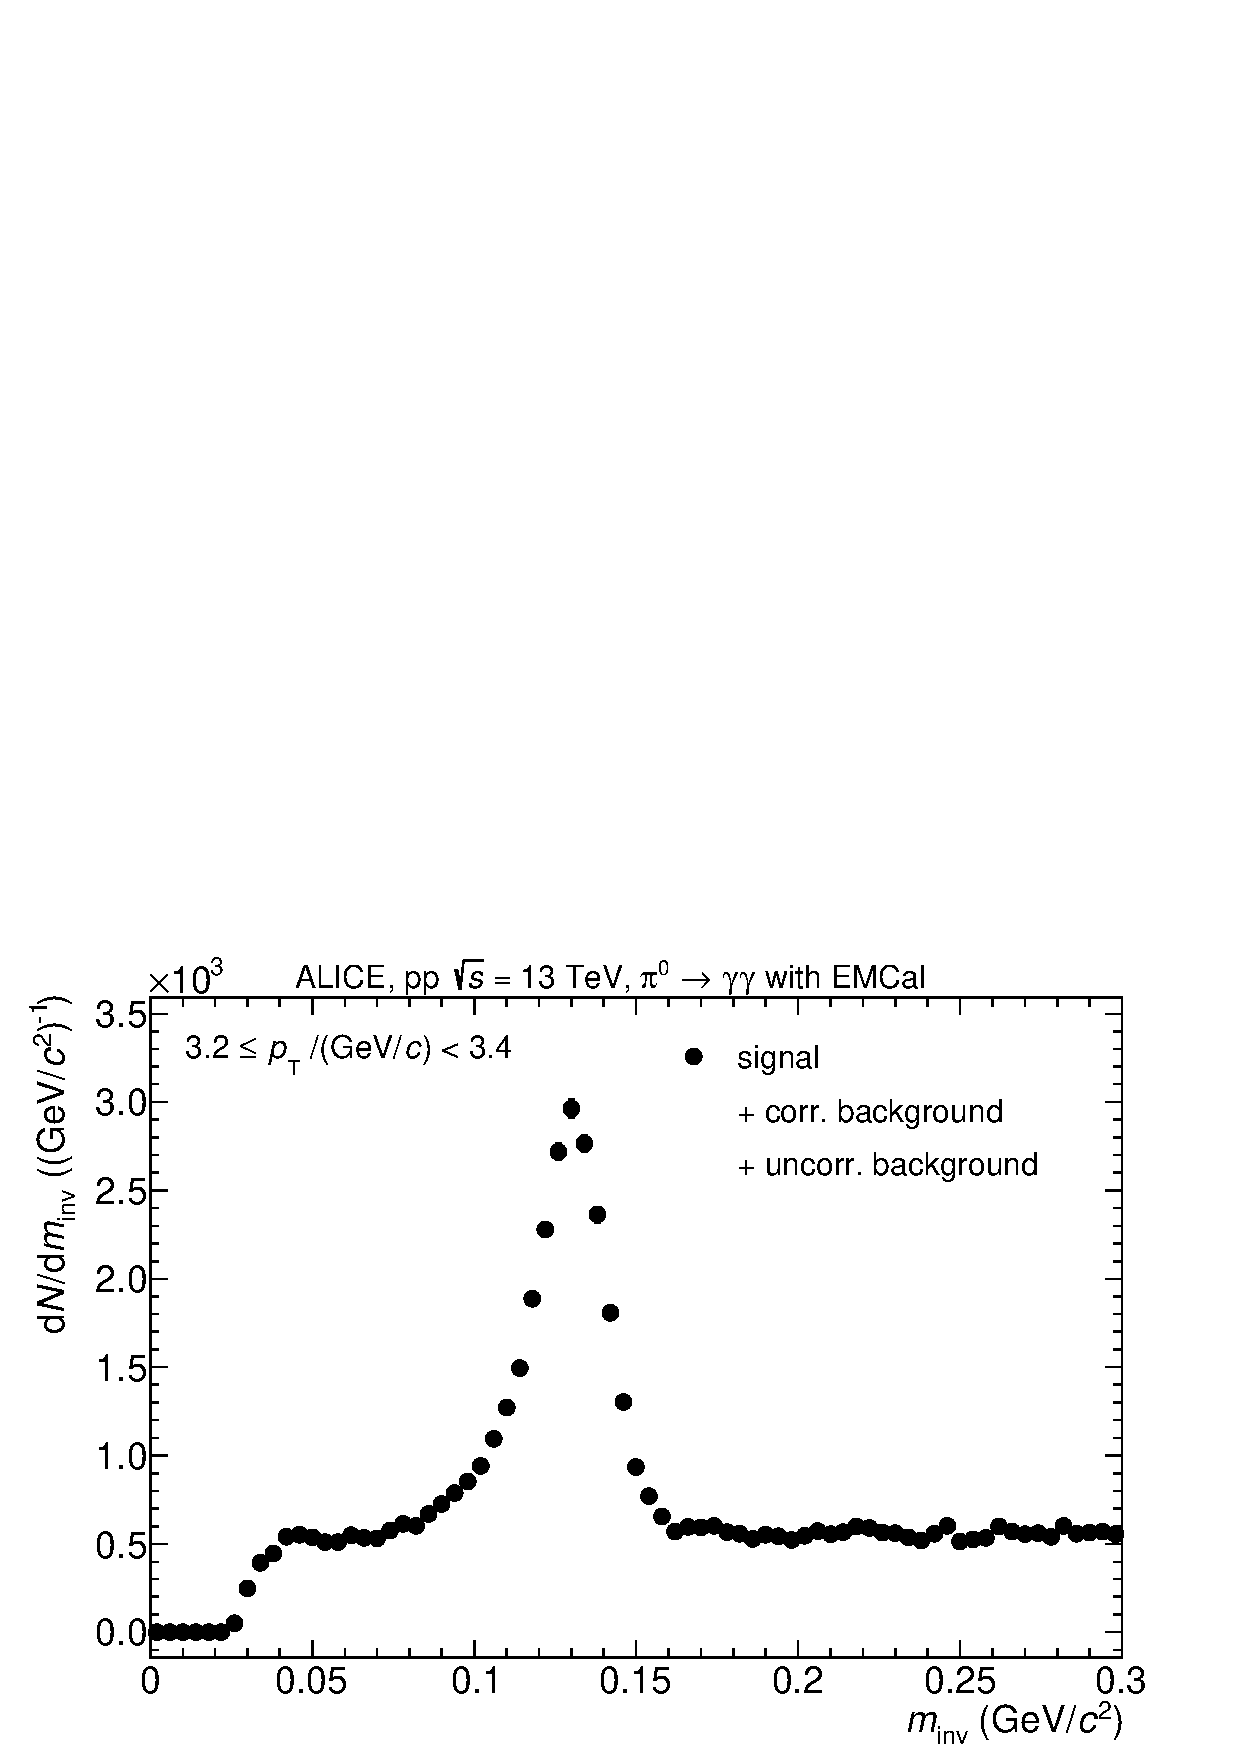
\includegraphics[width=.75\linewidth]{hSignalPlusBkg.pdf}
\caption{Projektion von Abbildung \ref{figInvMassPt_a} im $p_{\text{T}}$-Intervall $(3,2 - 3,4) (\text{GeV/}c)$. Es ist ein deutlicher Peak um $m_{\pi^{0}} \approx 0\,135\text{ GeV/}c^{2}$ zu erkennen, aber auch Untergrund, da das Signal zu höheren Massen gaußförmig abklingen sollte. Bei $m_{\text{inv}} < m_{\pi^{0}}$ kann Signal vorliegen, das aus konvertierten Photonen besteht, weshalb eine Aussage über die Form, beziehungsweise den Untergrund dort schwer möglich ist.}
\label{figSignalPlusBkg}
\end{figure}
\newline
Abbildung \ref{figSignalPlusBkg} zeigt die Anzahl der \textit{Clusterpaare} in Abhängigkeit der invarianten Masse im $p_{\text{T}}$-Intervall von $(3\,2 - 3\,4)(\text{GeV}/c)$.
Die in Abbildung \ref{figInvMassPt_a} beschriebene Anhäufung der Datenpunkten zeigt sich auch hier deutlich und wird im Folgenden als Peak bezeichnet.
Der Peak besteht wie zuvor erwähnt aus Signal.
\newline
Im folgenden Abschnitt wird eine Methode zur Abschätzung des unkorrelierten Untergrunds vorgestellt. 

\section{Absch{\"a}tzung des unkorrelierten Untergrunds} \label{s3s3}
\begin{figure}[tp]
\centering
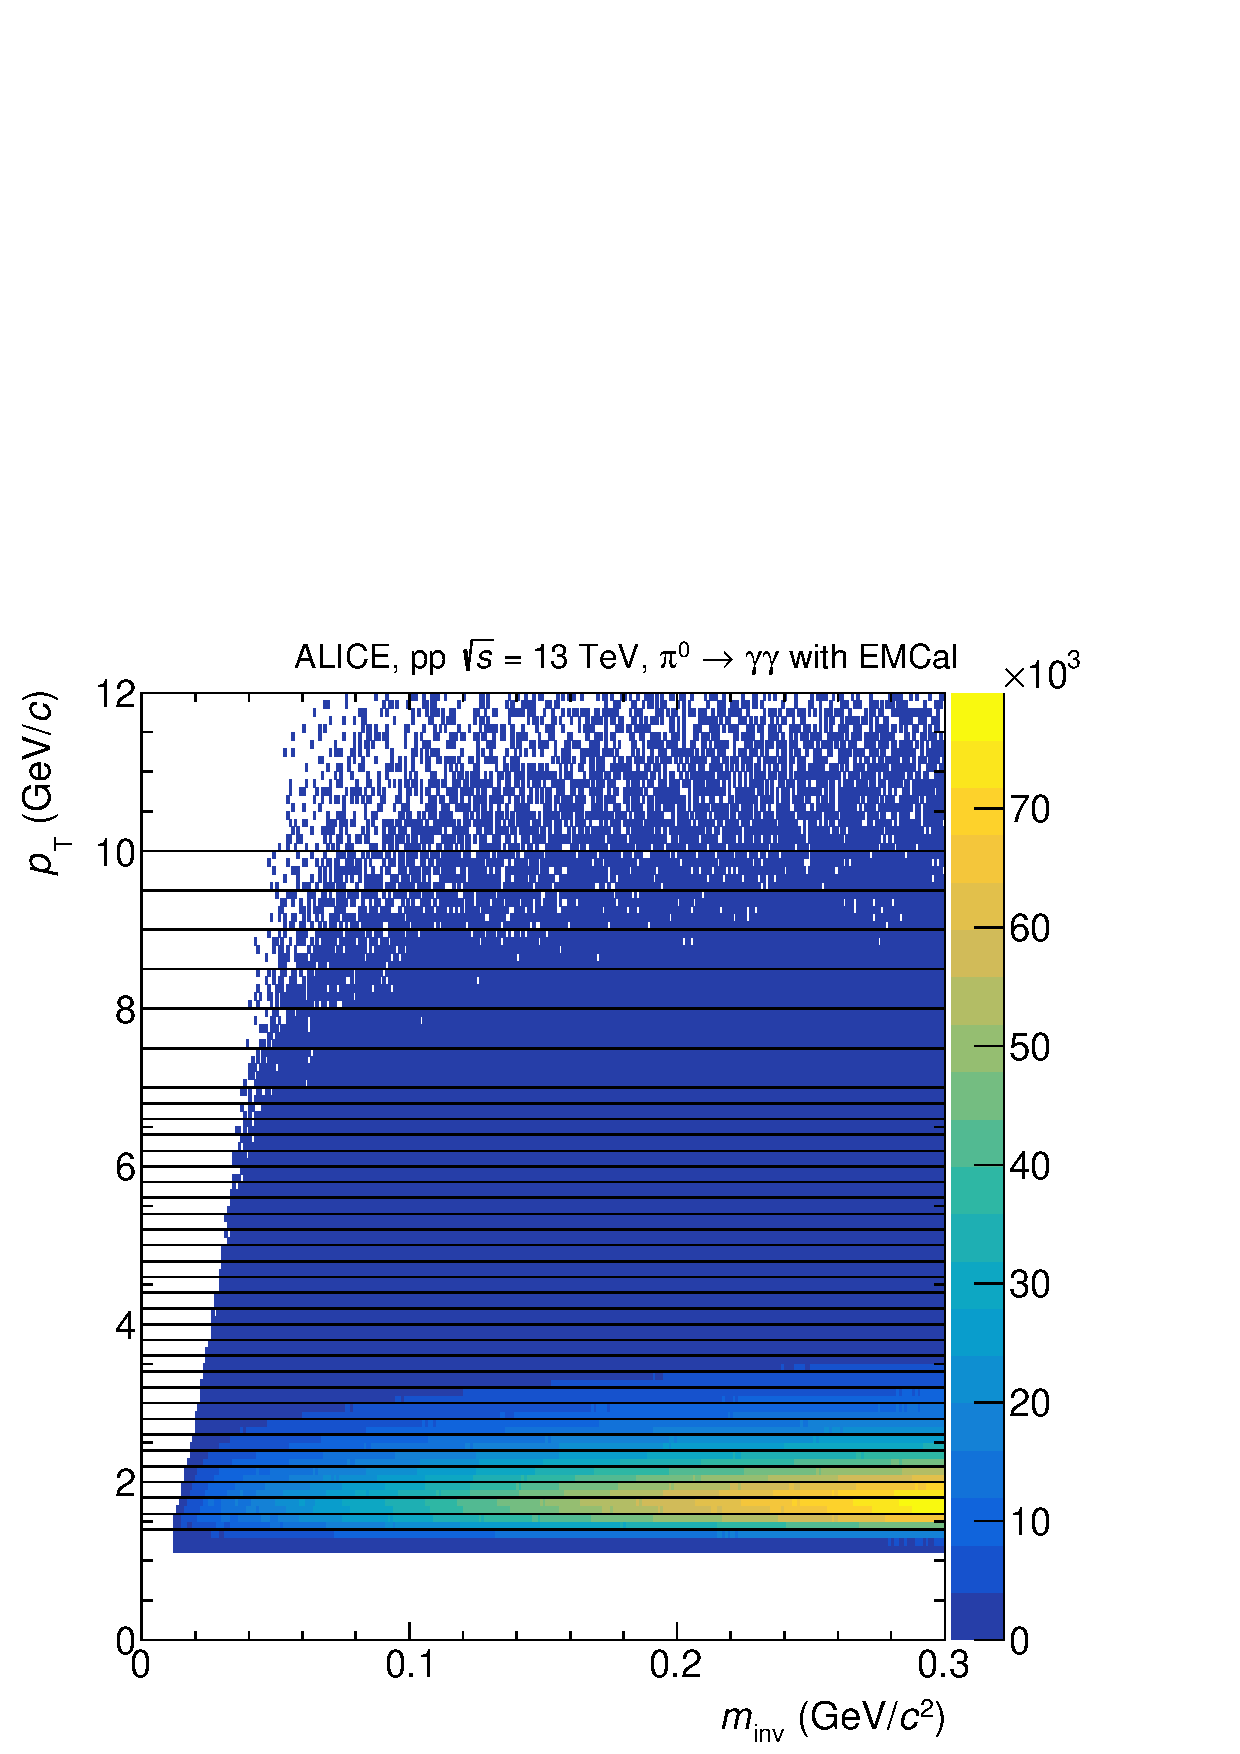
\includegraphics[width=.7\linewidth]{hInvMass_pT_Bkg.pdf}
\caption{$p_\text{T}$ und $m_\text{inv}$ als Funktion von der Anzahl von kombinierten  \textit{Clusterpaaren} aus unterschiedlichen \textit{events}.}
\label{figInvMassPt_b}
\end{figure}
Durch das paarweise Kombinieren aller Photonenkandidaten, wie es in Abschnitt \ref{s3s2} vorgestellt wurde, besteht ein großer Anteil der rekonstruierten Datenpunkte aus unkorreliert Paaren.
Um den unkorrelierten Untergrund abzuschätzen werden Photonenkandidaten aus unterschiedlichen \textit{events} paarweise miteinander kombiniert.
Dadurch wird sicher gestellt, dass zwischen den Photonenkandidaten keine Korrelation besteht.
Diese Methode wird als \textit{mixed event} Methode bezeichnet.
Abbildung \ref{figInvMassPt_b} zeigt eine Verteilung, bei der Photonenkandidaten aus unterschiedlichen \textit{events} miteinander kombiniert wurden.
Eine Häufung der Datenpunkte um eine bestimmte invariante Masse gibt es, wie zu erwarten, nicht.
Durch die Anforderungen an den Öffnungswinkel sind wieder keine Datenpunkte bei kleinen invarianten Massen zu finden.
Die untere Grenze der invarianten Masse, ab welcher Kombinationen möglich sind steigt mit $p_\text{T}$, analog wie zuvor bei Abbildung  \ref{figInvMassPt_a}.
\newline
In der \textit{mixed event} Methode gibt es eine größere Anzahl an Kombinationsmöglichkeiten, als in der \textit{same event} Methode.
Daraus resultiert eine größere Anzahl an Einträgen in der Verteilung der invarianten Masse und des Transversalimpulses, weshalb die Verteilung, die aus der \textit{mixed event} Methode kommt, skaliert werden muss an die Verteilung aus der \textit{same event} Methode.
Die Skalierung erfolgt bei $m_\text{inv} \in \left[0\,19,3\,0\right] (\text{GeV/}c^{2})$, da dort kein Signal erwartet wird.
Es ergibt sich für den Skalierungsfaktor:
\begin{align}
\label{eqBackSkalierung}
\alpha &= \frac{\sum_{i \neq j}\sum_{n}m_{\text{inv}}\left( \gamma^{(n)}_{i},\gamma^{(n)}_{j}\right) }{\sum_{i,j}\sum_{n \neq m}m_{\text{inv}}\left( \gamma^{(n)}_{i},\gamma^{(m)}_{j}\right) }
\end{align}
Die oberen Indize $m$ und $n$ stehen hierbei für ein Event, aus dem ein Photon kommt und die unteren Indize $i$ und $j$ numerieren die Photonen ($\gamma$).
\begin{figure}[tp]
\centering
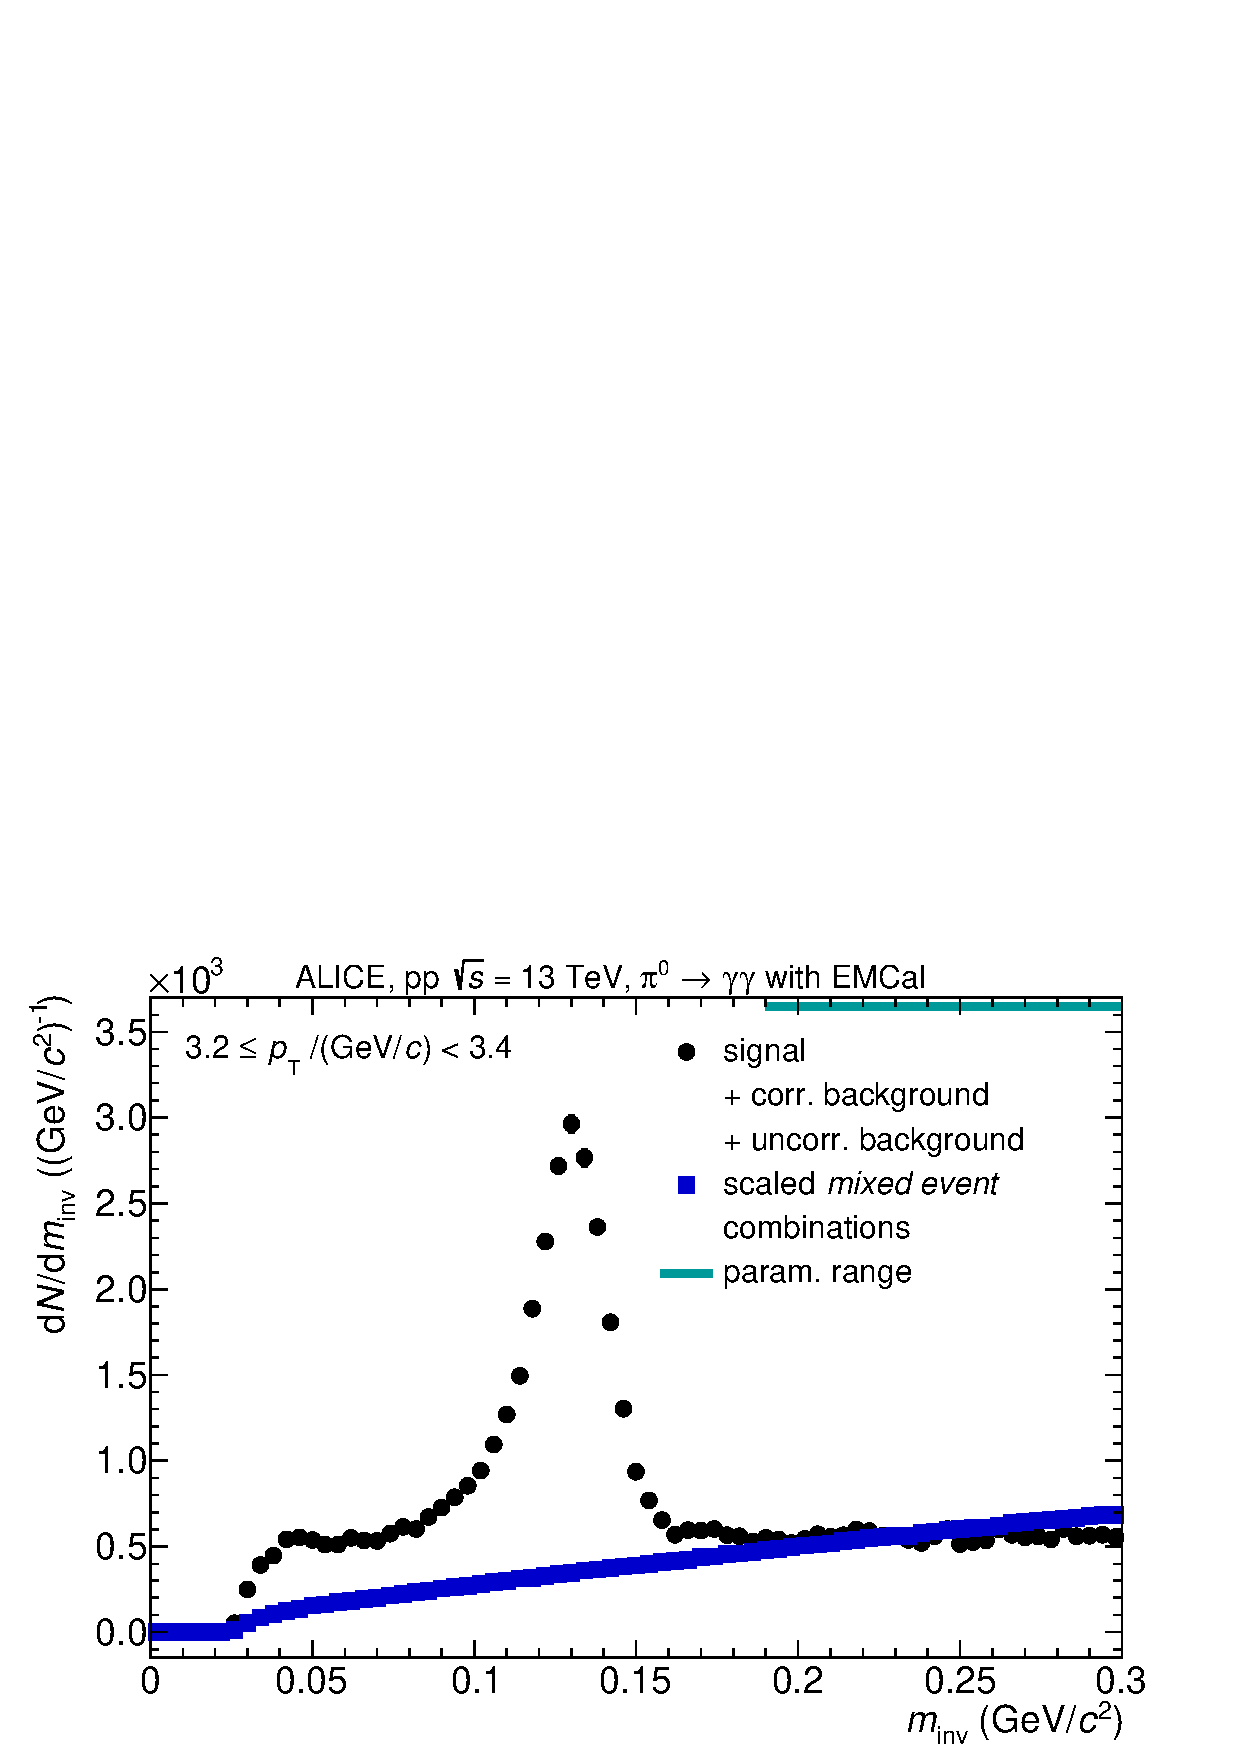
\includegraphics[width=.75\linewidth]{hUncorrBkgNorm.pdf}
\caption{Nach Gleichung \ref{eqBackSkalierung} skalierte {\it mixed event} Kombinationen als Abschätzung des unkorrelierten Untergrunds zusammen aufgetragen mit Signal zuzüglich beiden Untergrundkomponenten wie in Abbildung \ref{figSignalPlusBkg}.}
\label{figUncorrBkgNorm}
\end{figure}
\newline
Abbildung \ref{figUncorrBkgNorm} zeigt die skalierten \textit{mixed event} Kombinationen und das Signal zusammen mit dem korrelierten und dem unkorrelierten Untergrund.
Nachdem der unkorrelierte Untergrund abgeschätzt wird, wird dieser von der Verteilung der invarianten Masse aus der \textit{same event} Methode subtrahiert.
\begin{figure}[tp]
\centering
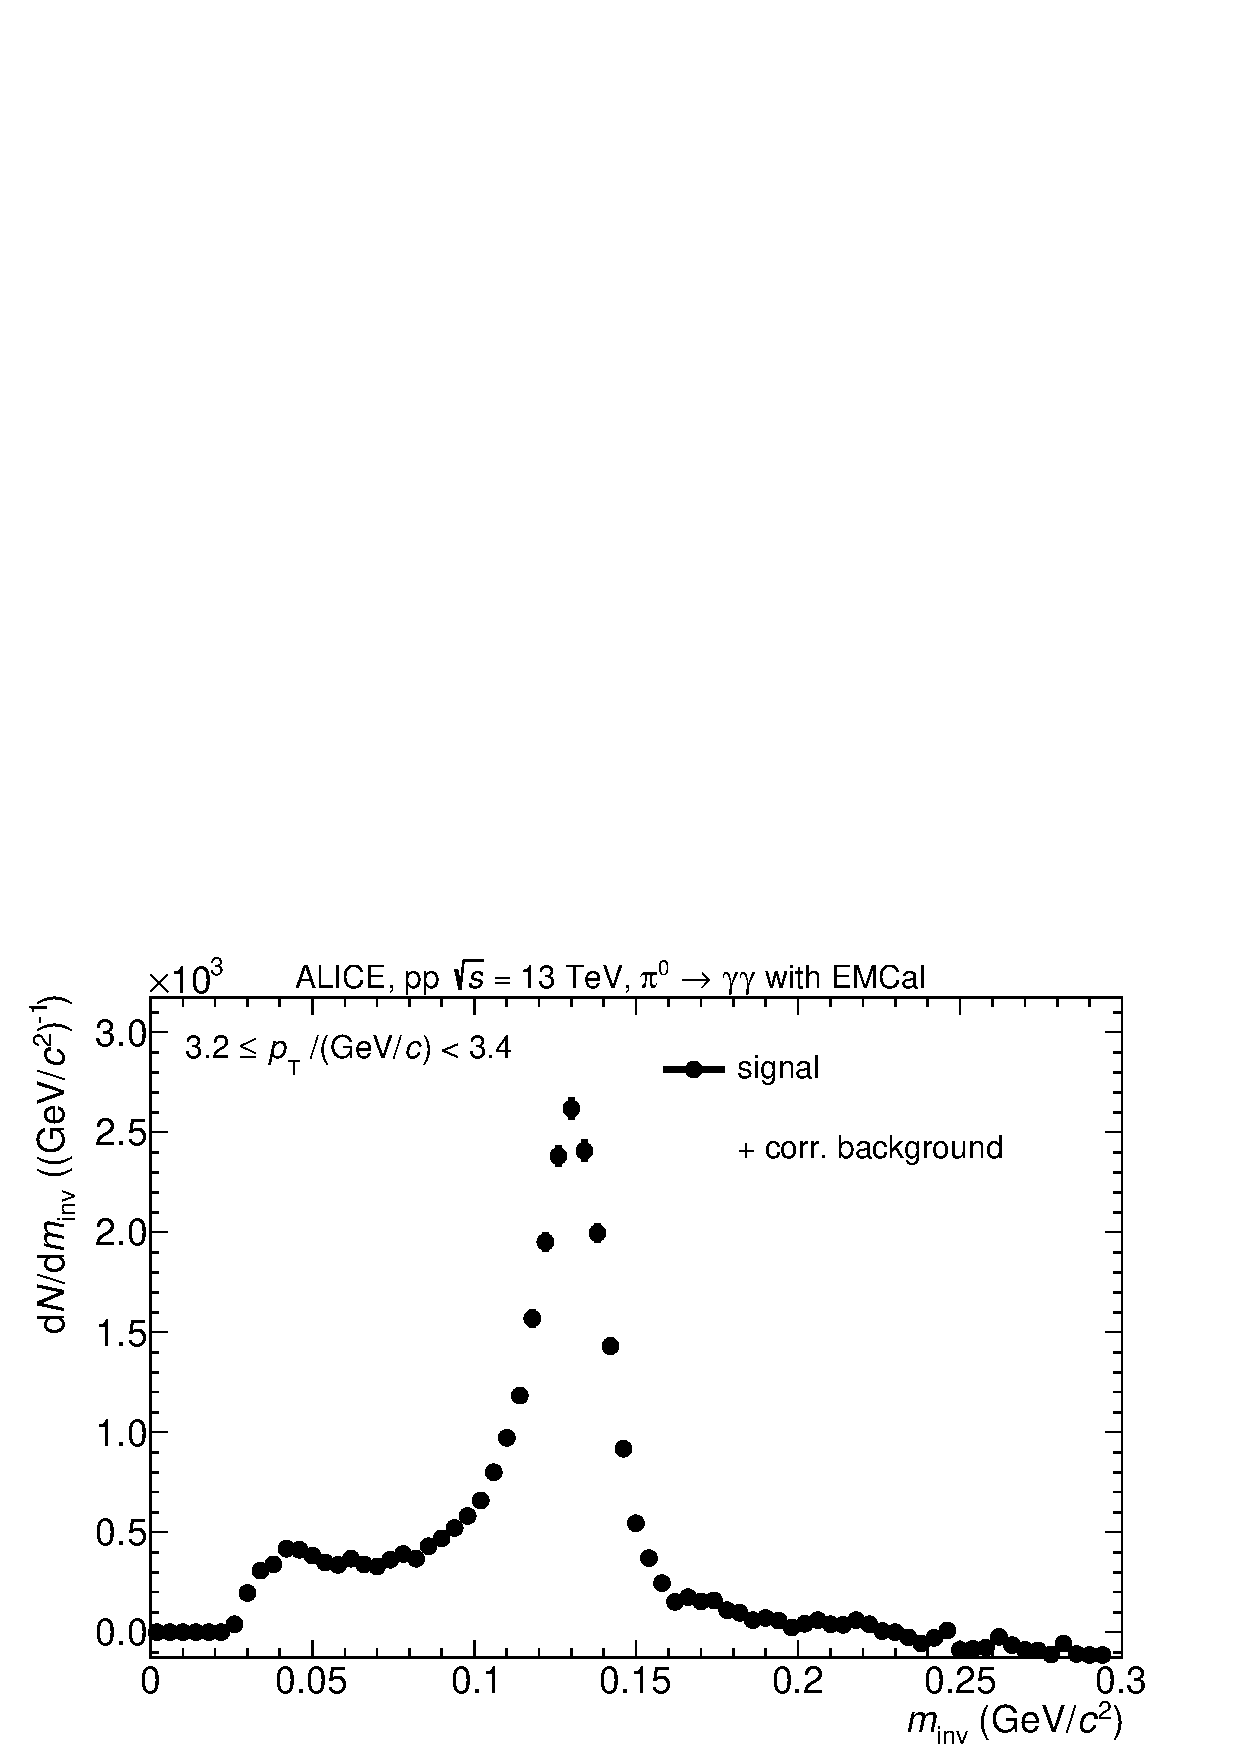
\includegraphics[width=.75\linewidth]{hInvMass_Data.pdf}
\caption{Signal nach Abzug des unkorrelierten Untergrunds.}
\label{figInvMass_Data}
\end{figure}
\newline
Abbildung \ref{figInvMass_Data} zeigt eine Verteilung der invarianten Masse aus der \textit{same event} Methode, nachdem die skalierten Kombinationen aus der \textit{mixed event} Methode, als Abschätzung der unkorrelierten Untergrunds, abgezogen wurden.
Durch die Subtraktion geht jegliche Information verloren, welche Photonenkandidatenpaare welchen Datenpunkt bilden.
Grund dafür ist, dass nicht einzelne Datenpunkte abgezogen werden, sonder lediglich eine gewisse Anzahl an Einträgen.
Deshalb spiegelt die Verteilung eine statistische Auswertung wider, mit statistischen Unsicherheiten.
\newline
Der nächste Schritt in der Analyse neutraler Pionen ist die Bestimmung des korrelierten Untergrunds.
Das Abschätzen mit einer linearen Funktion hat sich als gängigste Methode zur Abschätzung des korrelierten Untergrunds entwickelt und wird im Folgenden als Standardmethode bezeichnet.
In dieser Arbeit wird der korrelierte Untergrund sowie das reine $\pi^{0}$-Signal mit Hilfe von Monte Carlo Templates bestimmt.
Die Ergebnisse der Analyse mit Hilfe von Monte Carlo Templates, sowie mit der Standardmethode werden miteinander vergleichen, um eine Aussage über den möglichen Nutzen von Analysen mit Hilfe von Monte Carlo Templates treffen zu können.
Im folgenden Abschnitt wird zunächst die Standardmethode kurz erläutert.

\section{Absch{\"a}tzung des korrelierten Untergrunds mit der Standardmethode} \label{s3s4}
Da es sich bei dem Signal ohne Konversionsanteil um eine statistische Größe handelt, wird eine gaußförmig Funktion benutzt, um dieses zu beschreiben.
\newline
Der Konversionsanteil des Signals wird als \textit{Tail} Komponente bezeichent.
Diese Komponente wird durch eine exponentielle Funktion und einer gaußförmige Funktion beschrieben.
Sie dient der Abschätzung des Anteils des Signals, dem Konversionselektronen oder Konversionspositronen zu Grunde liegen.
Für die Abschätzung des korrelierten Untergrunds wird eine lineare Funktion angenommen.
Die drei Funktionen werden kombiniert an die Verteilung der invarianten Masse angepasst.
\begin{figure}[tp]
\centering
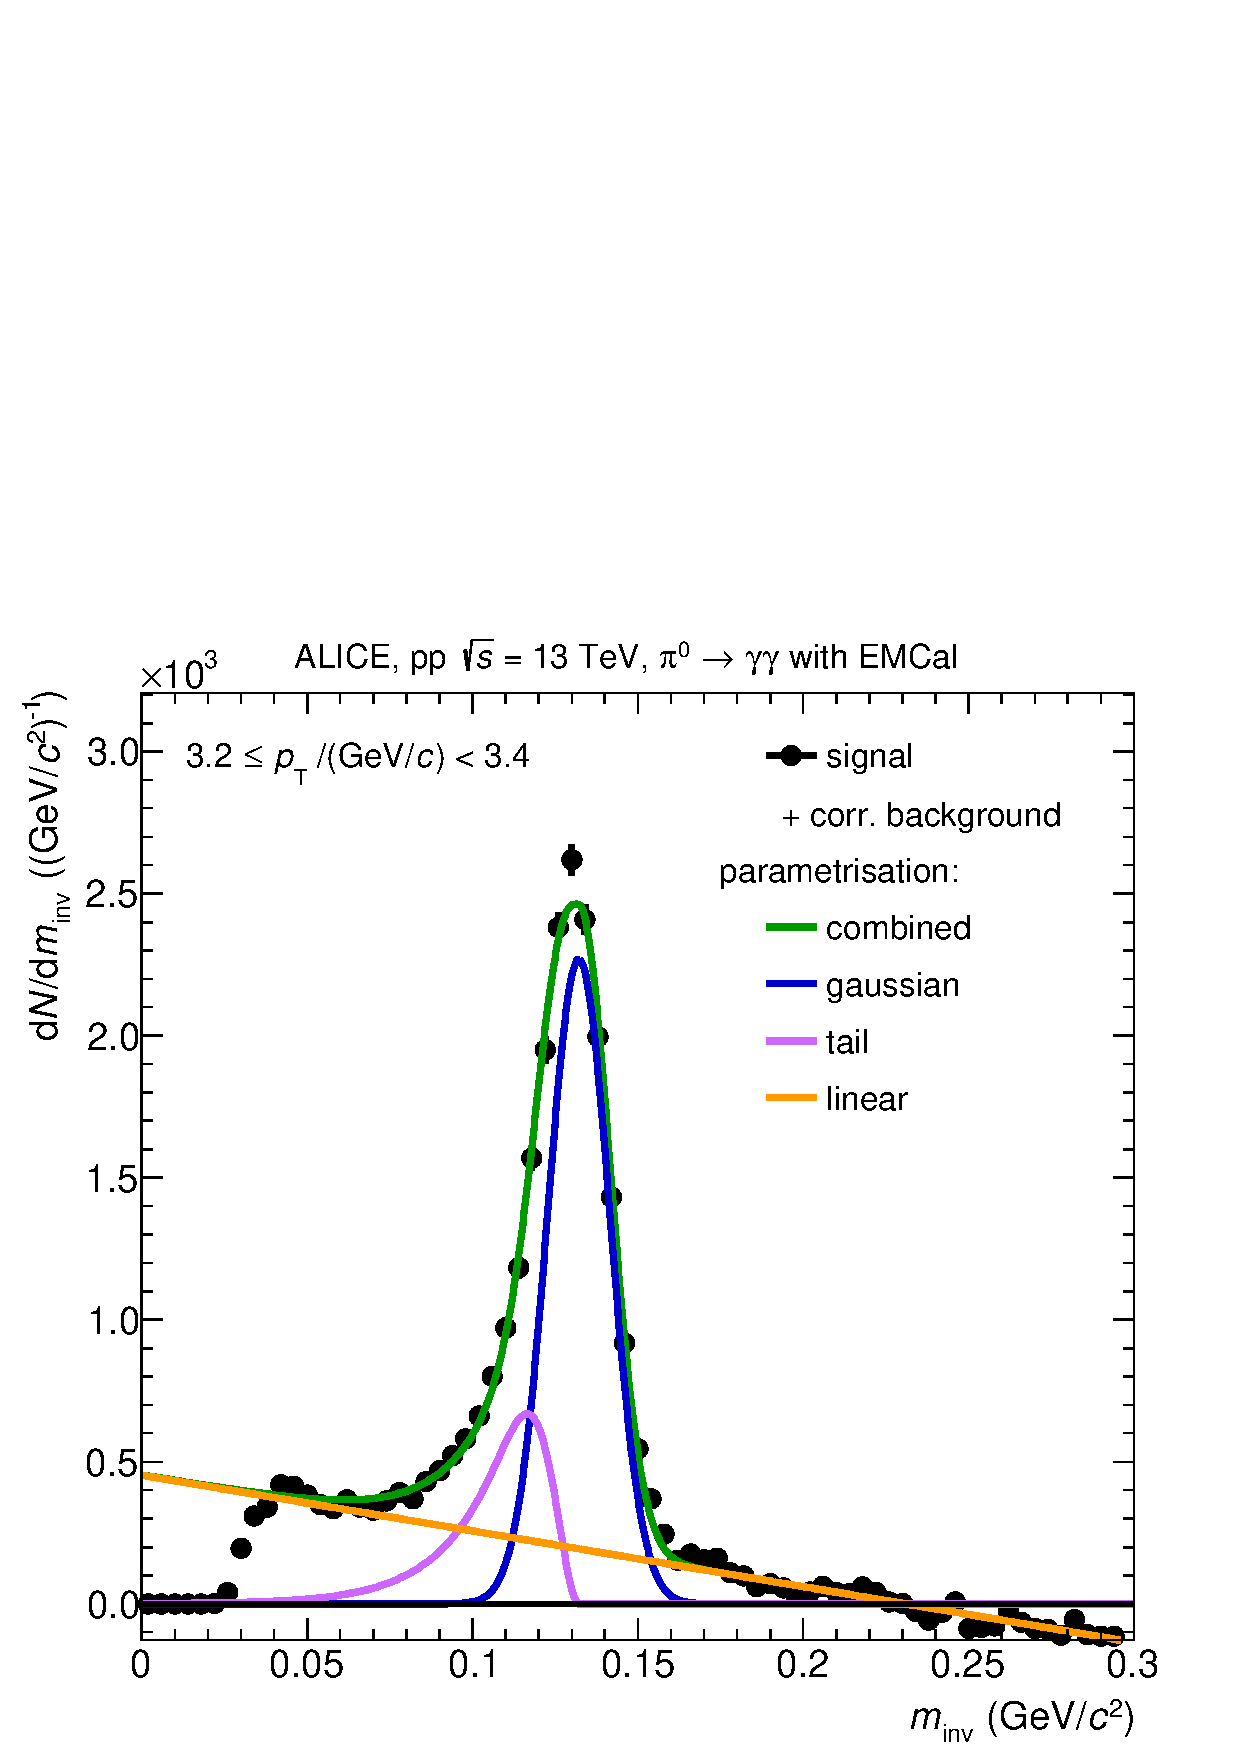
\includegraphics[width=.75\linewidth]{StandardParam.pdf}
\caption{Signal mit korreliertem Untergrund sowie den Funktionen zur Beschreibung des Signals mit korreliertem Untergrund.}
\label{figStandardParam}
\end{figure}
\newline
Abbildung \ref{figStandardParam} zeigt die Verteilung der invarianten Masse, bestehend aus Signal und korreliertem Untergrund, sowie das Ergebnis der an die Daten angepassten Funktion.
Die grüne Funktion entspricht der Summe der drei einzelnen Komponenten, wobei die Gauß-Funktion in blau, die \textit{Tail}-Funktion in pink und die lineare Funktion in orange dargestellt sind.
Dabei wird deutlich, dass durch die Abschätzung des korrelierten Untergrunds über die lineare Funktion bei $m_\text{inv} < 0\,06\text{ GeV}/c^{2}$ kein Signal erwartet wird.
Für $m_\text{inv} < 0\,02\text{ GeV}/c^{2}$ gibt es keine Einträge in der Verteilung aufgrund des minimalen Öffnungswinkels.
Dieses Verhalten wird nicht von der Abschätzung des korrelierten Untergrunds berücksichtigt.
\newline
Um die Anzahl der produzierten $\pi^{0}$ mit der Standardmethode zu bestimmen, wird die Anzahl der Einträge, die unter der lineare Parametrisierung liegen, von der Summe der Einträge der Daten abgezogen.
Anschließend werden die übrigen Daten, also das Signal, über einen festen Bereich um den Erwartungswert der Gauß-Funktion integriert.
Für eine detaillierte Beschreibung der Standardmethode sei an dieser Stelle auf \cite{thesis:Adrian} verwiesen.
\newline
Im folgenden Abschnitt wird die Abschätzung des korrelierten Untergrunds mit Hilfe von Templates beschrieben.

\section{Peakextraktion mit Hilfe von Parametrisierungen von Templates} \label{s3s5}
Um das Signal mit Hilfe von Templates zu extrahieren wird, wie auch bei der Standardmethode, zunächst eine Abschätzung des korrelierten Untergrunds gemacht.
Hierfür werden je $p_\text{T}$-Intervall zwei Templates an die Daten angepasst.
Das eine Template wird verwendet um das Signal, das zweite um den korrelierten Untergrund zu beschreibe.
\newline
Im folgenden Abschnitt wird das Template des Signals diskutiert. 

\subsection{Template des Signals} \label{s3s5s1}
Das Template des Signals wird mit Hilfe der Information der Monte Carlo Simulation erstellt.
Dabei wird ausgenutzt, dass in der Simulation bekannt ist, welchen Ursprung welches Teilchen hat und welches Teilchen auf das EMCal trifft.
Dadurch wird ermöglicht, genau bestimmen zu können, ob ein Photonkandidat aus dem Zerfall eines $\pi^{0}$ oder einem anderen Prozess stammt und ob es sich dabei um ein Photon, ein konvertiertes Elektron oder Positron, oder ein anderes Teilchen handelt.
\begin{figure}[tp]
\centering
\includegraphics[width=.75\linewidth]{PeakTemplateMotivation10_Data_2016.pdf}
\caption{Template des Signals (grün) mit seinen drei Teilkomponenten.
Diese bestehen aus Kombinationen mit zwei Photonen (blau), einem Photon und einem Konversionselektron oder Konversionspositron (gelb) und zwei unterschiedlichen Konversionselektronen oder Konversionspositronen (grau).}
\label{fig:SigTemp}
\end{figure}
\newline
%Joshuas Problem mit dem Satz?
Abbildung \ref{fig:SigTemp} zeigt das Template des Signals in grün, sowie die Aufteilung des Signals in seine einzelnen Komponenten.
%wording anders?
Die Komponenten setzen sich aus den drei möglichen Kombinationen von \textit{Clustern} zusammen.
Zum einen aus \textit{Clustern} aus Photonen, in der Abbildung als $\gamma$ bezeichnet, und zum anderen aus \textit{Clustern} aus einem Elektron oder Positron, die durch die Konversion  eines Photonen entstanden sind.
Letztere werden in der Abbildung durch $\gamma_\text{conv}$ symbolisiert.
\newline
In blau sind die Kombinationen aus zwei Photonen ($\gamma\gamma$) dargestellt, in gelb die Kombination aus Photon und Elektron oder Positron ($\gamma\gamma_\text{conv}$) und in grau die Kombination aus Konversionselektron oder Konversionspositron miteinander ($\gamma_\text{conv}\gamma_\text{conv}$).
\newline
Die Abbildung zeigt außerdem, wie zuvor angesprochen, dass bis $m_\text{inv}>0\,05 \text{ GeV}/c^{2}$ Signal vorliegt.
Der Anteil des Signals um diese invariante Masse besteht hauptsächlich aus zwei Teilchen einer Photonkonversion.
Genau dieser Teil des Signals wird nicht durch die Standardmethode berücksichtigt.
Durch das Berücksichtigen in der Analyse mit Hilfe der Templates kann ein größerer Anteil des Signals gezählt werden.
Deshalb wird eine geringere statistische Unsicherheit erwartet.

\subsection{Template des korrelierten Untergrunds} \label{s3s5s2}
F\"ur die Bestimmung des Templates des korrelierten Untergrunds wird das Template des Signals von einer Verteilung invarianter Masse abgezogen.
Die Verteilung invarianter Masse kommt dabei ebenfalls aus der Monte Carlo Simulation, auf die das Analyseverfahren bis einschlie{\ss}lich der Absch\"atzung der unkorellierten Untergrunds, so wie bisher erl\"autert, angewandt wurde.
\begin{figure}[tp]
\centering
\includegraphics[width=.75\linewidth]{EntstehungUntergrund10_Data_2016.pdf}
\caption{.}
\label{fig:BkgTemp}
\end{figure}
\newline
Abbildung \ref{fig:BkgTemp} zeigt das Template des korrelierten Untergrunds in pink.
Zur Verdeutlichung sind ebenfalls das oben beschriebene Signal in schwarz und das Template des Signals in gr\"un eingezeichnet.
\newline
Da die statistische Unsicherheit im korrelierten Untergrund relativ gro{\ss} ausf\"allt verglichen mit der Anzahl an Eintr\"agen in der Verteilung der invarianten Masse, wird in dieser Arbeit der korrelierte Untergrund aus mehreren $p_\text{T}$-Intervallen zusammengefasst.
Dabei werden die Templates des korrelierten Untergrunds aus den $p_\text{T}$-Intervallen von $p_\text{T} \beq 1,8\text{ GeV}/c$ bis $p_\text{T} \leq 2,8\text{ GeV}/c$ aufgrund der geringen statistischen Unsicherheit benutzt.
Diese werden zun\"achst aufsummiert und auf die Anzahl der verwendeten $p_\text{T}$-Intervalle normiert.
\begin{figure}[tp]
\centering
\includegraphics[width=.75\linewidth]{BackgroundWithRatio10_Data_2016.pdf}
\caption{.}
\label{fig:BkgTempRatio}
\end{figure}
\newline
Abbildung \ref{fig:BkgTempRatio} zeigt in pink ein kombiniertes Template des korrelierten Untergrunds und in gr\"un das Template des korrelierten Untergrunds f\"ur das $p_\text{T}$-Intervall $(3,2 - 3,4) (\text{GeV/}c)$.

\newline
Im Folgenden Abschnitt werden die beiden Templates so parametrisiert, dass sie das Signal nach Absch\"atzung des unkorrelierten Untergrunds bestm\"oglich beschreiben.

\subsection{Parametriesierungsmethode} \label{s3s5s3}
Parametrisierungsmethode:
Die Parametrisierung der beiden Templates erfolgt durch die sogenannte $\chi^{2}$-Minimierung.
$\chi^{2}$ gibt dabei als ein Ma{\ss} an, wie gut eine Verteilung an gegebene Daten passt.
Je kleiner $\chi^{2}$ ist, umso besser beschreibt die Verteilung die Daten, deshalb wird $\chi^{2}$ bei der Parametrisierung minimiert.
Als freie Parameter werden zwei Skalierungsfaktoren benutzt, einmal ein Skalierungsfaktor f\"ur das Template des Signals (SF\textsubscript{Signal}) und einmal ein Skalierungsfaktor f\"ur das Template des korrelierten Untergrunds (SF\textsubscript{korr. Untergrund}).
F\"ur $\chi^{2}$ gilt dann:
\begin{align}
\chi^{2} = \sum_{i}\left(\frac{ax_{i}}{•}\right)
\end{align}

\subsection{Abzug des korrelierten Untergrunds und Integration des Signals} \label{s3s5s4}
Das Ergebnis der Parametrisierung der Templates für das $p_\text{T}$-Intervall $(3\,2-3\,4)(\text{GeV/}c)$ wird in Abbildung \ref{KOMMT NOCH} dargestellt.
Die Parametrisierung der beiden Templates stimmt innerhalb der Unsicherheiten gut mit den Daten überein, wie zu erwarten war, nach Abbildung \ref{Chi2pT}.
%%detaillierter Beschreiben was man sieht?????
\newline
Um die Anzahl produzierter $\pi^{0}$ nun zu bestimmen, wird das skalierte Template des korrelierten Untergrunds von dem Signal ohne kombinatorischen Untergrund abgezogen.
Anschließend wird in einem bestimmten Zählbereich über die Werte des Signals summiert.
Dies wird für jedes $p_\text{T}$-Intervall durchgeführt.
\newline
Der Zählbereich hängt dabei von $p_\text{T}$ ab, da er so gewählt wurde, dass die untere Grenze immer groß genug ist, um nicht von den Anforderungen an den Öffnungswinkel betroffen zu sein.
Die obere Grenze liegt fest bei $p_\text{T} = 0\,25 \text{ GeV}/c$.
In Abbildung \ref{FEHLT} wird er Zählbereich durch eine blaue Linie markiert.
\newline
Das so erhaltene rohe Spektrum wird zusätzlich noch normiert, auf die Anzahl an \textit{events} $N_\text{evt}$, den Pseudorapiditätsbereich $\eta$, den Transversalimpuls $p_\text{T}$, die Wahrscheinlichkeit, dass ein $\pi^{0}$ in zwei Photonen zerfällt und $2\pi$.
Letzteres ist reine Konvention, während die anderen Normierungen einen Vergleich zwischen unterschiedlichen Analysen ermöglichen.
Abbildung \ref{FELHT AUCH NOCH!!!!!} zeigt eine normiertes rohes Spektrum.
Das Spektrum steigt zunächst leicht an, bis es bei $p_\text{T} = FEHLT NOCH\text{ GeV}/c$ sein Maximum erreicht.
Danach sinkt das Spektrum kontinuierlich.
\newline
Für eine genaue Aussage über die Produktionsrate von $\pi^{0}$ sowie einen allgemeinen Vergleich wird allerdings noch die Korrektur auf die Detektorakzeptanz sowie die Effizienz benötigt.

\chapter{Korrigierter Yield} \label{s4}

\section{Akzeptanz und Effizienz} \label{s4s1}
Die Korrekturen die auf das rohe Spektrum angewandt werden basieren auf der Monte Carlo Simulationen, aus der auch die Templates für diese Analyse stammen.
\newline
Die Detektorakzeptanz spiegelt dabei die Abdeckung des EMCals wider.
Sie berechnet sich aus dem Verhältnis der \textit{Clusterpaare}, die auf das EMCal treffen, zu den produzierten \textit{Clusterpaaren}.
\newline
Die Effizienz berechnet sich aus der Division der \textit{Clusterpaare} aus dem Template des Signals geteilt durch die Anzahl der akzeptierten \textit{Clusterpaaren}.
Für die Effizienz wird der $m_\text{inv}$ Bereich zum Zählen benutzt, der auch für die Bestimmung des rohen Spektrums benutzt wurde.
\begin{figure}[t]
\centering
\includegraphics[width=.65\linewidth]{Korrekturfaktoren_Data_2016.pdf}
\caption{Detektorakzeptanz und Effizienz in Abhängigkeit von $p_\text{T}$.
}
\label{fig:Korrekturen}
\end{figure}
\newline
Durch das Korrigieren des rohen Spektrums mit der Detektorakzeptanz und der Effizienz, wird die Anzahl der detektierten und extrahierten $\pi^{0}$ auf die Anzahl der produzierten $\pi^{0}$ korrigiert.
Abbildung \ref{fig:Korrekturen} zeigt die beiden Korrekturgrößen Detektorakzeptanz und Effizienz.
\newline
Zerfällt ein $\pi^{0}$ in zwei Photonen, so fliegen die Photonen im System des $\pi^{0}$ entgegengesetzt zu einander weg, $\theta_{\gamma\gamma}$ beträgt in diesem System $180^{\circ}$.
Abhängig vom $p_\text{T}$ den ein $\pi^{0}$ im Laborsystem hat verringert sich $\theta_{\gamma\gamma}$.
Je größer $p_\text{T}$ umso kleiner $\theta_{\gamma\gamma}$.
Deshalb treffen beide Photonen aus einem $\pi^{0}$-Zerfall bei niedrigem $p_\text{T}$ seltener auf das EMCal.
Aus diesem Grund steigt die Detektorakzeptanz leicht an.
\newline
Durch die Anforderungen an die \textit{Cluster} werden unter anderem auch \textit{Cluster} ausgeschlossen, deren zugrunde liegende Teilchen aus dem Zerfall eines $\pi^{0}$ stammen, aber zu wenig Energie besitzen.
Gerade asymmetrische Zerfälle, bei denen der Anteil der zur Verfügung stehenden Energie ungleichmäßig auf die Zerfallsprodukte aufgeteilt wird, werden durch die Energieanforderung an die \textit{Cluster} ausgeschlossen.
Deshalb steigt die Effizienz bis $p_\text{T} \approx 8 \text{ GeV}/c$ an und saturiert dann.

\section{Systematische Unsicherheit} \label{s4s2}
Für den korrigierten Yield wird zu Letzt noch die systematische Unsicherheit bestimmt.
Dabei wird sich in dieser Arbeit rein auf die systematische Unsicherheit, die durch Variation in der Peakeextraktion kommt, fokussiert.
Die Variationen die in dieser Arbeit verwendet wurden lassen sich in vier Abschnitte unterteilen.
\newline
Bei der \textbf{Variation des Zählbereiches}, wird der Zählbereich einmal ausgeweitet und ein anderes mal verkleinert.
Für das Verkleinern wird dabei der untere Wert für $m_\text{inv}$ um $0\,01 \text{ GeV}/c^{2}$ erhöht, während der obere Wert für $m_\text{inv}$ um $0\,025 \text{ GeV}/c^{2}$ verringert wird.
Entsprechend wird beim Ausweiten der untere Wert für $m_\text{inv}$ um $0\,025 \text{ GeV}/c^{2}$ verringert der obere Wert für $m_\text{inv}$ um $0\,025 \text{ GeV}/c^{2}$ erhöht.
Bei der \textbf{Variation des Parametrisierungsbereiches} wird analog verfahren, mit den gleichen Zahlenwerten.
\newline
Die \textbf{Variation der Templates des korrelierten Untergrunds} basiert auf den in Abschnitt \ref{s3s5s2} vorgestellten Methoden zur Bestimmung der Templates des korrelierten Untergrunds.
%Text + Bild
\begin{table}[b!]
\centering
\begin{tabular}{c|c|c|}
\cline{2-3}
                                                          & $\Delta m_\text{inv}$ $\left(\text{GeV}/c^{2}\right)$ & $p_\text{T}$-Intervall $\left(\text{GeV}/c\right)$ \\ \hline
\multicolumn{1}{|c|}{\multirow{3}{*}{Standard}}           & $0\,004$                                              & $1\,4-7\,5$                                        \\ \cline{2-3} 
\multicolumn{1}{|c|}{}                                    & $0\,008$                                              & $7\,5-10$                                          \\ \cline{2-3} 
\multicolumn{1}{|c|}{}                                    & $0\,010$                                              & $10-12$                                            \\ \hline \hline
\multicolumn{1}{|c|}{\multirow{3}{*}{Vergr{\"o}{\ss}ert}} & $0\,005$                                              & $1\,4-7\,5$                                        \\ \cline{2-3} 
\multicolumn{1}{|c|}{}                                    & $0\,010$                                              & $7\,5-10$                                          \\ \cline{2-3} 
\multicolumn{1}{|c|}{}                                    & $0\,016$                                              & $10-12$                                            \\ \hline \hline
\multicolumn{1}{|c|}{\multirow{3}{*}{Verkleinert}}        & $0\,002$                                              & $1\,4-7\,5$                                        \\ \cline{2-3} 
\multicolumn{1}{|c|}{}                                    & $0\,005$                                               & $7\,5-10$                                          \\ \cline{2-3} 
\multicolumn{1}{|c|}{}                                    & $0\,008$                                              & $10-12$                                            \\ \hline
\end{tabular}
\caption{Die verschiedenen Breiten der $m_\text{inv}$-Intervalle $\Delta m_\text{inv}$ in Abhängigkeit von $p_\text{T}$.}
\label{tab:Binning}
\end{table}
\newline
Als letztes wird noch die Breite der $m_\text{inv}$-Intervalle $\Delta m_\text{inv}$ in der \textbf{Variation des Rebinnings} verändert.
Die Werte für $\Delta m_\text{inv}$ hängen zunächst von zwei Faktoren ab.
Zum einen werden die Daten für die Analyse in $800$ gleichgroße $m_\text{inv}$-Intervalle aufgeteilt, die von $m_\text{inv} = 0\,0 \text{ GeV}/c^{2}$ bis $m_\text{inv} = 0\,8 \text{ GeV}/c^{2}$ reichen.
Somit beträgt $\Delta m_\text{inv}$ anfangs immer $0\,001 \text{ GeV}/c^{2}$.
Dieser Wert wird vergrößert um die statistische Unsicherheit möglichst klein zu halten, wobei darauf geachtet werden muss, dass es sich bei dem Faktor, um den $\Delta m_\text{inv}$ vergrößert wird, um einen gemeinsamen Teiler von $800$ handelt.
Tabelle \ref{tab:Binning} zeigt $\Delta m_\text{inv}$ im Normalfall, sowie für beide Variationen.
Dabei hängt $\Delta m_\text{inv}$ zusätzlich von $p_\text{T}$ ab.
\newline
Die gesamte Systematische Unsicherheit ergibt sich aus dem quadratischen Mittelwert der mittleren systematischen Unsicherheiten der vier Variationsarten.

\section{Vergleich mit Standardmethode} \label{s4s3}
\begin{figure}[t!]
\centering
\includegraphics[width=.65\linewidth]{KorrigierteYields_Data_2016.pdf}
\caption{Korrigierte $p_\text{T}$-Spektren aus der Template Methode sowie aus der Standardmethode.
Außerdem das Verhältnis der beiden Spektren.}
\label{fig:KorrYieldComp}
\end{figure}
Abbildung \ref{fig:KorrYieldComp} zeigt das korrigierte $p_\text{T}$-Spektrum aus der Template Methode zusammen mit dem korrigierte $p_\text{T}$-Spektrum aus der Standardmethode.
Außerdem zeigt die Abbildung das Verhältnis von ersterem zu letzterem.
Das Verhältnis zeigt eine Diskrepanz zwischen den beiden Spektren von durchschnittlich etwa $3\%$ auf.
Im Bereich von $3,8 \leq p_\text{T}/\text{ (GeV}/c) < 5,8$ liegt das Verhältnis innerhalb der statistischen Unsicherheiten auf $1$.
Der größte Unterschied zwischen den Spektren beträgt etwa $10\%$, wo die statistischen Unsicherheiten der beiden Spektren den Unterschied nicht abdecken.
Mit Hilfe der systematischen Unsicherheit neben den statistischen Unsicherheit sollte sich eine gute Übereinstimmung der beiden Spektren ergeben.
\begin{figure}[t!]
\centering
\includegraphics[width=.65\linewidth]{StatistischeUnsicherheitVergleich_Data_2016.pdf}
\caption{Statistische Unsicherheit der korrigierten $p_\text{T}$-Spektren aus der Analysemethode mit Templates, sowie aus der Standardmethode in Abhängigkeit von $p_\text{T}$.}
\label{fig:StatUncer}
\end{figure}
\newline
Abbildung \ref{fig:StatUncer} zeigt die statistischen Unsicherheiten der Spektren der beiden Methoden.
Der Verlauf der statistischen Unsicherheiten weist große Ähnlichkeit auf.
Über fast den gesamten $p_\text{T}$-Bereich hat die Template Methode eine geringe statistische Unsicherheit, als die Standardmethode.
Die geringere statistische Unsicherheit bei der Template Methode kommt von dem großen Zählbereich, der mit  dieser Methode möglich ist, sowie aus dem Konversionsanteil des Signals.
Zuvor wurde bereits gezeigt, dass die Standardmethode diesen Anteil des Signals unterschätzt.
\newline
Aufgrund der geringeren statistischen Unsicherheit der Template Methode, sowie der guten Über\-ein\-stim\-mung mit der Standardmethode stellt die Tempalte Methode eine mögliche Alternative zur Standardmethode dar.
Dabei kann sie entweder als neuer Standard für die Analyse von $\pi^{0}$ in pp-Kollisionen benutzt werden, oder als eine Variation für die Bestimmung der systematischen Unsicherheiten.
%\newline
%Außerdem zeigt der Vergleich der beiden Methoden, dass die Produktion von $\pi^{0}$ in pp-Kollisionen theoretisch gut verstanden wurde, da die Templates aus einer Monte Carlo Simulation entstanden.

\chapter{Zusammenfassung und Ausblick} \label{s5}
In der vorliegenden Arbeit werden Daten von pp-Kollisionen bei $\sqrt{s}=13\text{ TeV}$ analysiert.
Die Daten sind im Jahr 2016 mit dem ALICE-Experiment aufgezeichnet worden.
Bei der Analyse handelt es sich um eine Analyse neutraler $\pi^{0}$ aus Messungen des EMCals.
\newline
Zunächst werden die Zellen des EMCals, die Energie gespeichert haben, zu \textit{Clustern} zusammengefasst.
Um \textit{Cluster}, denen Photonen zugrunde liegen, von anderen \textit{Clustern} zu unterscheiden, werden verschiedene Anforderungen an die \textit{Cluster} gestellt.
Die so selektierten \textit{Clustern} werden anschließend in der \textit{same Event} Methode paarweise miteinander kombiniert und der Transveralsimpuls sowie die invariante Masse der \textit{Clusterpaare} berechnet.
\newline
Die daraus entstandene Verteilung der invarianten Masse und des Transversalimpulses besteht aus rekonstruierten $\pi^{0}$ und Untergrund.
Der Untergrund teilt sich in zwei Komponenten auf, den korrelierten und den unkorrelierten Untergrund.
Um den unkorrelierten Untergrund abzuschätzen wurden \textit{Cluster} aus unterschiedlichen Events in der \textit{mixed Event} Methode miteinander kombiniert und skaliert.
\newline
Im Rahmen dieser Analyse werden die Verteilungen in 35 $p_\text{T}$-Intervalle aufgeteilt und einzeln betrachtet.
Die skalierte Verteilung der invarianten Masse aus der \textit{mixed Event} Methode wird von der Verteilung der invarianten Masse aus der \textit{mixed Event} abgezogen.
\newline
Die verbleibende Verteilung wird in dieser Arbeit durch Templates beschrieben.
Die Templates werden mit Hilfe einer Monte Carlo Simulation erzeugt.
Für jedes $p_\text{T}$-Intervall wird dabei ein eigenes Template des Signals verwendet, während es ein global benutztes Template des korrelierten Untergrunds gibt.
Das Template des korrelierten Untergrunds wird mit Hilfe einer speziell für diesen Zweck angepassten Monte Carlo Simulation an die einzelnen $p_\text{T}$-Intervalle angepasst.
Diese Anpassung wird benötigt, da die Anforderung an den Öffnungswinkel zwischen zwei Photonen in einer $p_\text{T}$ abhängige untere Grenze für $m_\text{inv}$ resultiert.
\newline
Um die Templates an die Daten anzupassen werden diese mittels $\chi^{2}$-Minimierung parametrisiert.
Das skalierte Template des korrelierten Untergrunds, das aus der Parametrisierung kommt, wird von der Verteilung der invarianten Masse der Daten ohne unkorrelierten Untergrund subtrahiert.
Die übrige Verteilung der Daten, das Signal wird anschließend über einen festen $m_\text{inv}$-Bereich integriert und damit die Anzahl rekonstruierter $\pi^{0}$ in Abhängigkeit von $p_\text{T}$ bestimmt.
\newline
Das so extrahierte $p_\text{T}$-Spektrum wird anschließend auf die Detektorakzeptanz und die Rekonstruktionseffizienz korrigiert.
Durch Variationen in der Signalextraktion wird anschließend die systematische Unsicherheit im korrigierten $p_\text{T}$-Spektrum bestimmt.
\newline
Abschließend wird das korrigierte $p_\text{T}$-Spektrum aus der Analyse mit Hilfe von Monte Carlo Templates verglichen mit dem korrigierten $p_\text{T}$-Spektrum der Analyse mit Hilfe von Funktionsparametrisierung.
Die Abweichung der beiden Spektren liegt im $5\%$ Bereich und das Verhältnis der beiden Spektren ist innerhalb der statistischen Unsicherheit einigermaßen mit $1$ vereinbar.
Zuletzt wird die statistische Unsicherheit der beiden Analysemethoden verglichen.
Dabei zeigt sich, dass die Analyse mit Hilfe von Monte Carlo Templates fast in allen $p_\text{T}$-Intervallen geringere statistische Unsicherheiten hat, als die andere Analysemethode.
\newline
Für einen vollständigen Vergleich der beiden Methoden wird noch die systematische Unsicherheit der Analyse mit Funktionsparametrisierung benötigt.
Außerdem kann die Analyse mit Tempaltes noch erweitert werden, indem der unkorrelierte Untergrund ebenfalls durch die Verwendung eines Templates zusammen mit dem Template des Signals und dem Templates des korrelierten Untergrunds parametrisiert wird.
\clearpage

\appendix
\chapter{} \label{Appendix:A}
\begin{table}[h]
	\centering

\begin{tabular}{ | c || r | r ||  l  || c || r | r | }
		\hline
		$p_\text{T} \text{ (GeV}/c)$ & Integral & Unsicherheit & \ & $p_\text{T} \text{ (GeV}/c)$ & Integral & Unsicherheit \\ \hline
		1,4 - 1,6 & 8183,77 \  & 248,36 \hspace{3mm}  & \ &  5,0 - 5,2 & 375,78 \ & 76,18 \hspace{3mm} \\ \hline
		1,6 - 1,8 & 12696,80 \ & 319,21 \hspace{3mm} & \ &  5,2 - 5,4 & 183,20 \ & 70,98 \hspace{3mm} \\ \hline
		1,8 - 2,0 & 14928,40 \ & 335,82 \hspace{3mm} & \ &  5,4 - 5,6 & 273,14 \ & 64,85 \hspace{3mm} \\ \hline
		2,0 - 2,2 & 13686,40 \ & 323,90 \hspace{3mm} & \ &  5,6 - 5,8 & 105,55 \ & 61,23 \hspace{3mm} \\ \hline
		2,2 - 2,4 & 10766,10 \ & 300,70 \hspace{3mm} & \ &  5,8 - 6,0 & 106,59 \ & 56,42 \hspace{3mm} \\ \hline
		2,4 - 2,6 & 9047,53 \  & 273,67 \hspace{3mm} & \ &  6,0 - 6,2 & 34,35 \  & 52,23 \hspace{3mm} \\ \hline
		2,6 - 2,8 & 6901,65 \  & 246,32 \hspace{3mm} & \ &  6,2 - 6,4 & 3,41 \   & 49,94 \hspace{3mm} \\ \hline
		2,8 - 3,0 & 5429,20 \  & 221,03 \hspace{3mm} & \ &  6,4 - 6,6 & 8,73 \   & 46,40 \hspace{3mm} \\ \hline
		3,0 - 3,2 & 4220,52 \  & 198,67 \hspace{3mm} & \ &  6,6 - 6,8 & -23,16 \ & 43,73 \hspace{3mm} \\ \hline
		3,2 - 3,4 & 3253,74 \ & 178,66 \hspace{3mm} & \ &  6,8 - 7,0 & -13,32 \ & 40,78 \hspace{3mm} \\ \hline
		3,4 - 3,6 & 2660,09 \ & 160,66 \hspace{3mm} & \ &  7,0 - 7,5 & -47,53 \ & 56,97 \hspace{3mm} \\ \hline
		3,6 - 3,8 & 1994,75 \ & 144,91 \hspace{3mm} & \ &  7,5 - 8,0 & -35,33 \ & 49,50 \hspace{3mm} \\ \hline
		3,8 - 4,0 & 1537,27 \ & 130,91 \hspace{3mm} & \ &  8,0 - 8,5 & -79,79 \ & 42,67 \hspace{3mm} \\ \hline
		4,0 - 4,2 & 1411,16 \ & 118,39 \hspace{3mm} & \ &  8,5 - 9,0 & -85,09 \ & 39,43 \hspace{3mm} \\ \hline
		4,2 - 4,4 & 852,25 \  & 108,17 \hspace{3mm} & \ &  9,0 - 9,5 & -39,02 \ & 35,48 \hspace{3mm} \\ \hline
		4,4 - 4,6 & 817,07 \  & 99,02 \hspace{3mm} &  \ &  \ 9,5 - 10,0 & -32,65 \ & 31,98 \hspace{3mm} \\ \hline
		4,6 - 4,8 & 590,26 \  & 89,73 \hspace{3mm} &  \ &  10,0 - 12,0 & -288,32 \ & 50,04 \hspace{3mm} \\ \hline
		4,8 - 5,0 & 460,15 \  & 82,49 \hspace{3mm} &  \ & \   & \  & \  \\ \hline
	
\end{tabular}
	
\caption{Integral und Unsicherheit der Templates des korrelierten Untergrunds für die verschiedenen $p_\text{T}$-Intervalle.}
\label{tab:IntAndError}
\end{table}
\clearpage

\begin{figure*}[t]
\centering
\begin{multicols}{2}
    \includegraphics[width=.65\linewidth]{Anhang/BackgroundWithRatio01_Data_2016.pdf}\par 
    \includegraphics[width=.65\linewidth]{Anhang/BackgroundWithRatio02_Data_2016.pdf}\par 
\end{multicols}
\begin{multicols}{2}
    \includegraphics[width=.65\linewidth]{Anhang/BackgroundWithRatio03_Data_2016.pdf}\par
    \includegraphics[width=.65\linewidth]{Anhang/BackgroundWithRatio04_Data_2016.pdf}\par
\end{multicols}
\begin{multicols}{2}
    \includegraphics[width=.65\linewidth]{Anhang/BackgroundWithRatio03_Data_2016.pdf}\par
    \includegraphics[width=.65\linewidth]{Anhang/BackgroundWithRatio04_Data_2016.pdf}\par
\end{multicols}
\begin{multicols}{2}
    \includegraphics[width=.65\linewidth]{Anhang/BackgroundWithRatio05_Data_2016.pdf}\par
    \includegraphics[width=.65\linewidth]{Anhang/BackgroundWithRatio06_Data_2016.pdf}\par
\end{multicols}
\end{figure*}
\clearpage

\begin{figure*}[t]
\centering
\begin{multicols}{2}
    \includegraphics[width=.65\linewidth]{Anhang/BackgroundWithRatio07_Data_2016.pdf}\par 
    \includegraphics[width=.65\linewidth]{Anhang/BackgroundWithRatio08_Data_2016.pdf}\par 
\end{multicols}
\begin{multicols}{2}
    \includegraphics[width=.65\linewidth]{Anhang/BackgroundWithRatio09_Data_2016.pdf}\par
    \includegraphics[width=.65\linewidth]{Anhang/BackgroundWithRatio11_Data_2016.pdf}\par
\end{multicols}
\begin{multicols}{2}
    \includegraphics[width=.65\linewidth]{Anhang/BackgroundWithRatio12_Data_2016.pdf}\par
    \includegraphics[width=.65\linewidth]{Anhang/BackgroundWithRatio13_Data_2016.pdf}\par
\end{multicols}
\begin{multicols}{2}
    \includegraphics[width=.65\linewidth]{Anhang/BackgroundWithRatio14_Data_2016.pdf}\par
    \includegraphics[width=.65\linewidth]{Anhang/BackgroundWithRatio15_Data_2016.pdf}\par
\end{multicols}
\end{figure*}
\clearpage

\begin{figure*}[t]
\centering
\begin{multicols}{2}
    \includegraphics[width=.65\linewidth]{Anhang/BackgroundWithRatio16_Data_2016.pdf}\par 
    \includegraphics[width=.65\linewidth]{Anhang/BackgroundWithRatio17_Data_2016.pdf}\par 
\end{multicols}
\begin{multicols}{2}
    \includegraphics[width=.65\linewidth]{Anhang/BackgroundWithRatio18_Data_2016.pdf}\par
    \includegraphics[width=.65\linewidth]{Anhang/BackgroundWithRatio19_Data_2016.pdf}\par
\end{multicols}
\begin{multicols}{2}
    \includegraphics[width=.65\linewidth]{Anhang/BackgroundWithRatio20_Data_2016.pdf}\par
    \includegraphics[width=.65\linewidth]{Anhang/BackgroundWithRatio21_Data_2016.pdf}\par
\end{multicols}
\begin{multicols}{2}
    \includegraphics[width=.65\linewidth]{Anhang/BackgroundWithRatio22_Data_2016.pdf}\par
    \includegraphics[width=.65\linewidth]{Anhang/BackgroundWithRatio23_Data_2016.pdf}\par
\end{multicols}
\end{figure*}
\clearpage

\begin{figure*}[t]
\centering
\begin{multicols}{2}
    \includegraphics[width=.65\linewidth]{Anhang/BackgroundWithRatio01_Data_2016.pdf}\par 
    \includegraphics[width=.65\linewidth]{Anhang/BackgroundWithRatio02_Data_2016.pdf}\par  %NEEDS TO BE CHANGED
\end{multicols}
\begin{multicols}{2}
    \includegraphics[width=.65\linewidth]{Anhang/BackgroundWithRatio03_Data_2016.pdf}\par
    \includegraphics[width=.65\linewidth]{Anhang/BackgroundWithRatio04_Data_2016.pdf}\par
\end{multicols}
\begin{multicols}{2}
    \includegraphics[width=.65\linewidth]{Anhang/BackgroundWithRatio03_Data_2016.pdf}\par
    \includegraphics[width=.65\linewidth]{Anhang/BackgroundWithRatio04_Data_2016.pdf}\par
\end{multicols}
\begin{multicols}{2}
    \includegraphics[width=.65\linewidth]{Anhang/BackgroundWithRatio03_Data_2016.pdf}\par
    \includegraphics[width=.65\linewidth]{Anhang/BackgroundWithRatio04_Data_2016.pdf}\par
\end{multicols}
\end{figure*}
\clearpage

\begin{figure*}[t!]
\begin{multicols}{2}
	\centering
    \includegraphics[width=.65\linewidth]{Anhang/BackgroundWithRatio01_Data_2016.pdf}\par 
    \includegraphics[width=.65\linewidth]{Anhang/BackgroundWithRatio02_Data_2016.pdf}\par 
\end{multicols}
\caption{Vergleich der Templates des korrelierten Untergrunds aus den restlichen $p_\text{T}$-Intervallen mit dem kombinierten Template des korrelierten Untergrunds.}
\label{fig:OtherRatios}
\end{figure*}
\clearpage


%\begin{figure}
%\begin{subfigure}{.5\textwidth}
%  \centering
%  \includegraphics[width=.8\linewidth]{Anhang/BackgroundWithRatio01_Data_2016.pdf}
%\end{subfigure}%
%\begin{subfigure}{.5\textwidth}
%  \centering
%  \includegraphics[width=.8\linewidth]{Anhang/BackgroundWithRatio01_Data_2016.pdf}
%\end{subfigure}
%\caption{plots of something}
%\label{fig:fig}
%\end{figure}
\newpage
\bibliography{bib_bath_mahe} 
\bibliographystyle{alpha}
\clearpage
\chapter{Danksagung} \label{Appendix:B}
Zuallererst möchte ich mich bei Prof. Dr. Henner Büsching bedanken, der mich in seiner Gruppe aufgenommen hat und mir dadurch ermöglicht hat, diese Arbeit schreiben zu können.
Er stand jederzeit für Fragen zur Verfügung, sowohl bezüglich physikalischer Natur, als auch bei Fragen bezüglich des Schreibens.
\newline
Mein weiterer Dank gilt Fabian Pliquett, der zusammen mit Prof. Dr. Büsching viel Zeit aufgewandt hat, um mir unter anderem die Bedeutung von Präzision und Konsistenz näher zu bringen, dir mir nicht nur für diese Arbeit, sondern auch für mein weiteres Arbeitsleben nützlich sein wird.
\newline
Neben Fabian möchte ich mich auch bei meiner Bürokollegin Kristina Schmitt und meinen Büro\-kol\-le\-gen Sebastian Scheid, Patrick Reichelt und Janik Ditzel bedanken, die für ein angenehmes Arbeitsklima gesorgt haben, in zweifacher Hinsicht.
\newline
Weiterhin möchte ich mich bei meinem Betreuer Joshua König bedanken, der von Anfang an ein offenes Ohr für alle meine Fragen hatte und mir stets Anregungen gegeben hat, wenn ich mal nicht weiter wusste.
\newline
Außerdem hat Joshua zusammen mit Adrian Mechler mir den Einstieg in die Arbeitsgruppe sowie in das Arbeiten mit C++ und root erleichtert, weshalb auch ihm Dank gebührt.
\newline
Mein Dank gilt auch Andrea Hornung, die mir, wie Joshua, sowohl bei Fragen bezüglicher der Analyse, als auch bei Fragen rund ums Schreiben geholfen hat.
\newline
Weiterhin möchte ich mich bei der gesamten Hochenergiephysik-Gruppe am IKF bedanken, die mich freundlich aufgenommen und mir hilfreiches Feedback für meine Arbeit gegeben hat sowie für einige schöne Momente gesorgt hat.
\newline 
Ein großer Dank gilt auch meiner Familie, die mir unter der Präsumtion, dass ich mein Studium erfolgreich abschließen kann, sowohl moralisch als auch finanziell zur Seite steht und durch deren Unterstützung mein Studium überhaupt erst möglich wurde.
\newline
Zuletzt möchte ich mich noch bei meinen Freunden Florian Zindel, Katharina Zoch, Jan Röder und Julia Lienert bedanken, die mich während des Studiums und vor allem während des Schreibens dieser Arbeit unterstützt haben.

\end{document}
